\documentclass{article}
\usepackage[utf8]{inputenc}
\usepackage{graphicx}
\usepackage{algorithm}
\usepackage{algorithmic}
% \usepackage{algcompatible}

\usepackage{algpseudocode}
\usepackage{appendix}
\usepackage[margin=1.25in]{geometry} % Size of margin
\usepackage{hyperref} % Hyperlinks
\usepackage{tcolorbox} % Highlighting important concepts
\usepackage{setspace}
% Font Selection
\usepackage{fontspec}
\setmainfont{Arial}
% Bibliography
% \usepackage[
% backend=biber,
% style=alphabetic,
% ]{biblatex}
% \title{A bibLaTeX example}
% \addbibresource{bibliography.bib} %Imports bibliography file
% WORD COUNT COMMANDS
\usepackage{verbatim}
\usepackage{pdflscape}
% Font Size
\documentclass[10pt]{book}

\newcommand{\detailtexcount}[1]{%
  \immediate\write18{texcount -merge -sum -q #1.tex output.bbl > #1.wcdetail }%
  \verbatiminput{#1.wcdetail}%
}

\newcommand{\quickwordcount}[1]{%
  \immediate\write18{texcount -1 -sum -merge -q #1.tex output.bbl > #1-words.sum }%
  \input{#1-words.sum} words%
}

\newcommand{\quickcharcount}[1]{%
  \immediate\write18{texcount -1 -sum -merge -char -q #1.tex output.bbl > #1-chars.sum }%
  \input{#1-chars.sum} characters (not including spaces)%
}
% END OF WORD COUNT COMMANDS

% Defining Function for indenting formatting of functions
\newlength\myindent
\setlength\myindent{2em}
\newcommand\bindent{%
  \begingroup
  \setlength{\itemindent}{\myindent}
  \addtolength{\algorithmicindent}{\myindent}
}
\newcommand\eindent{\endgroup}
% End of definitions


\begin{document}

% Double Line Spacing
\doublespacing

%TC:ignore
%Title Page
\begin{titlepage}
   \begin{center}
       \vspace*{0.5cm}
    \large
       \textbf{Development of a spatial navigation task using line-following robots}

       \vspace{0.5cm}
        Supervisors: \textbf{Prof. John O'Keefe} and \textbf{Dr. Jake Ormond}
            
       \vspace{1.5cm}

       \textbf{Alif Ul Aziz} \\
       Word Count: 3505
       \vfill
            
       A dissertation presented for the partial fulfilment of the degree of\\
       Intercalated Bachelor of Science Medical Sciences with Mathematics, Computers and Medicine
            
       \vspace{0.8cm}
     
       
\includegraphics[width=0.3\textwidth]{images/ucl_logo.png}
    
        \vspace{1 cm}
       University College London Medical School \\ \& Sainsbury Wellcome Centre\\
       United Kingdom\\
       April 2022
            
   \end{center}
\end{titlepage}

% WORDCOUNT DATA

% \quickwordcount{main}
% \quickcharcount{main}
% \detailtexcount{main}

% Abstract
\section*{Abstract}

\paragraph{Background}
The investigation of spatial memory is important in the understanding of effect spatial memory pathologies such as Alzheimer's Disease. The underlying mechanisms of spatial memory are investigated with animal models' ability to navigate in maze environments. 
There have been previous maze designs that have allowed the animal model to make a limited number of choices deciding where to navigate to. The Honeycomb Maze is able to make a significant improvement on this by allowing many more decisions to be made by the animal model as well as a greater number of parameters being measured in a single run 
\paragraph{Aim of this work}
The aim of this dissertation is to develop a version of the Honeycomb Maze which is formed of three platforms moving around a hexagonal grid of possible moves for the animal model to make. This was programmed in Python successfully for integration with preexisting libraries.

\paragraph{Solution}
A solution was programmed using object oriented paradigm programming. By investigating the geometry of the problem presented, a general path-finding solution was made for navigating through the maze, without collisions between robots taking place. This was integrated into a network of possible moves the robots can access without collision. From this the shortest path for each path-finding target is generated and executed by the robots.


\paragraph{Conclusion}
A path-finding solution, for the specific task presented, has been implemented for the \textit{Khepera IV} robots in Python. This allows its use as a tool for investigating animal models of spatial cognition. However, there are limitations in its efficiency which can be addressed upon further work.


% and here is why you should care


\pagebreak

%Contents
\tableofcontents
\pagebreak

\section*{Acknowledgements}

I am grateful to Prof. John O'Keefe for the opportunity to under take the project and would like to extend my gratitude to Dr Jake Ormond for supervising me on this project and providing constructive feedback on my work.

Further to this I would like to thank Dr Steven West on guidance for understanding the paradigm of object oriented programming as well as providing the space to discuss implementation details.

I would also like to extend my thanks to everyone 
in the O'Keefe Laboratory for being so generous with their time, resources as well as providing the environment for me to develop my critical thinking skills and academic intuition.
\pagebreak
%TC:endignore

%Introduction
\section{Introduction}

Spatial learning is an important function involved in navigation and the formation of episodic memories \cite{spatial_learning_memory}.
The hippocampus and medial entorhinal cortex are implicated for spatial learning due to the presence of the cells that are key for encoding space - namely cells such as the place cells (for coding locations), grid cells (for distance in a particular direction), head direction cells (heading direction) and boundary cells (for the boundaries of an environment).

\paragraph{Clinical Relevance}

There is evidence that in the early stages of Alzheimer's Disease (AD), visuo-spatial memory impairment \cite{Diagnosis}, is partly due to the degeneration of hippocampal cholinergic synaptic transmission \cite{Impairments}, which distinguishes it from other neuro-degenerative diseases.

% and is important in the differential diagnosis of AD.

With greater insight into spatial memory encoding in the hippocampal area, it could be possible to come up with a better understanding of how learning and memory functions, as well as developing improved early diagnosis of AD.

\paragraph{Previous Maze Designs}

Previously, there has been use of the Morris Water-Maze \cite{morris_water_maze} where a rodent is placed in the water and must navigate to find the platform just beneath the water and navigate towards it when placed in the water at different points.
The Radial Arm maze \cite{radial_arm_maze} is an improvement on the T shaped maze \cite{t-maze} which only has two choices for the animal to reach, whereas the radial arm maze allows one of 7 choices for the animal model, allowing higher resolution investigation into the cognitive map as a wider range of the parameters can be recorded.

\begin{figure}[h]
    \centering
    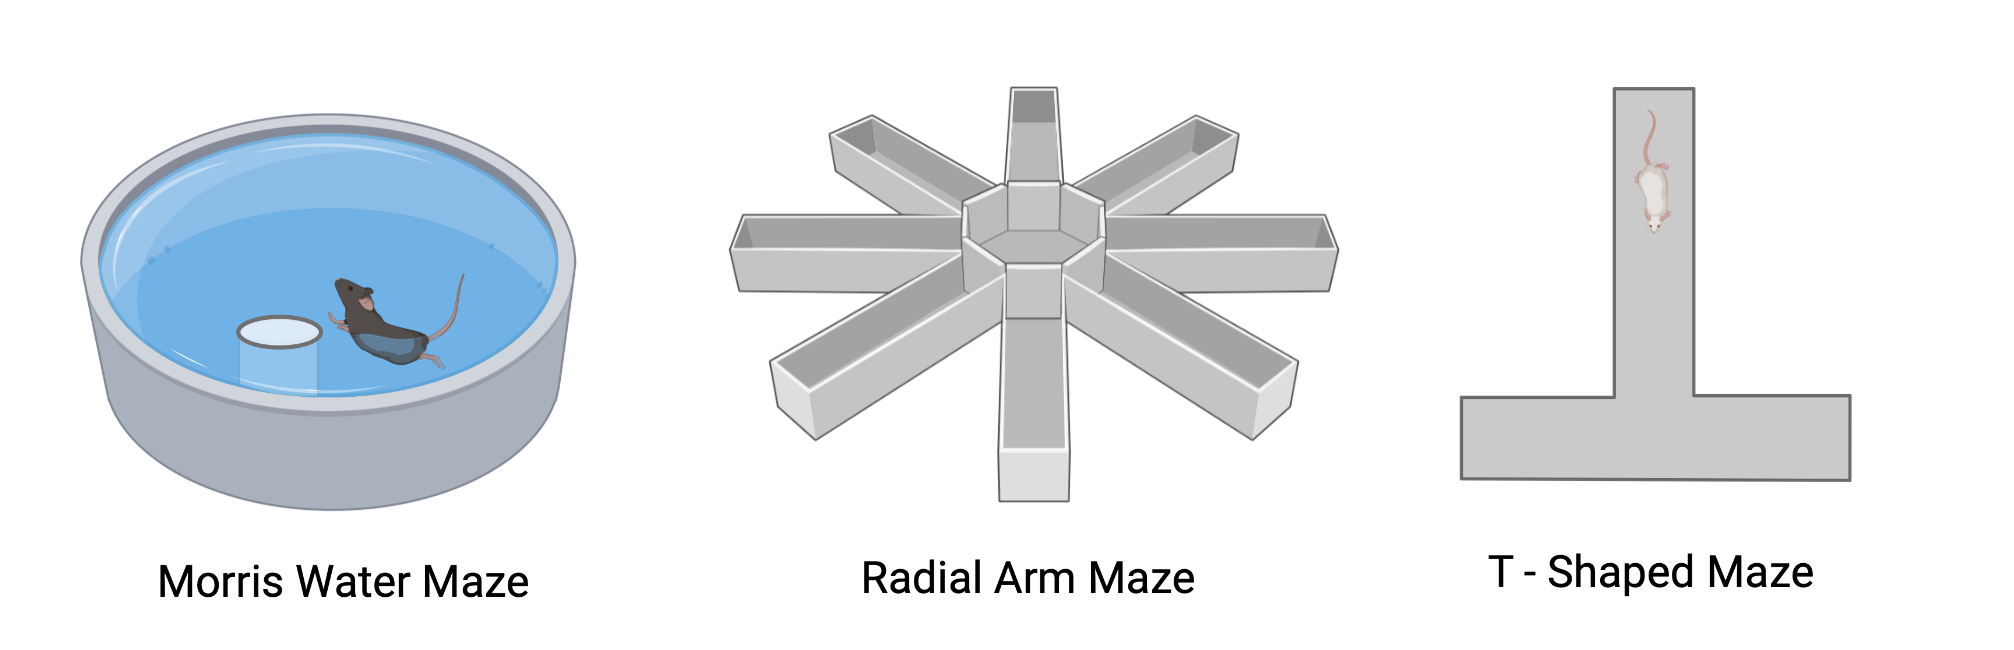
\includegraphics[scale=0.4]{images/previous_maze_designs.png}
    \caption{This figure shows previous designs of mazes used for investigating spatial memory of rodents.}
    \label{fig:previous_maze_designs}
\end{figure}

The important improvement that the Honeycomb Maze brings, is the ability to introduce many more choices for where the animal would like to move to: each time mouse is presented with a decision, it can choose between one of two possible choices.  Parameters such as angle of animal movement and distance to goal were also be correlated with the animals' navigation performance \cite{nature_honeycomb_maze_paper}. 

The Honeycomb Maze's makes is the ability to respond to the changing position of the animal poses a great advantage over static mazes such as the radial arm maze where the choices presented to the animal model are unchanging.
The Honeycomb Maze has been shown to be effective in investigating the cognitive maps of animal models \cite{nature_honeycomb_maze_paper} however, comes at the practical cost of building such a maze . This includes the financial cost of making the maze (approx. £100,000) in the laboratory as well as space required to do so, limiting movement choices for the animal.

The proposed solution is to use platform robots that are able to dynamically move around each-other to offer choices to the animal model. This design reduces the cost of building the maze to around £8,000. Further to this, the number of positions the animal model can navigate to is only limited by the size of the room not the relatively expensive cost of building more platforms from the previous design.

% \begin{tcolorbox}
\\

\paragraph{The aim of the dissertation} is to develop a tool for investigating behaviour of the animal models by implementing the Dynamic Honeycomb Maze Brief, providing a greater range of decisions the animal model can make.

% \end{tcolorbox}
\pagebreak

%Methods
\section{Design Brief and Method for the Dynamic Honeycomb Maze}



\subsection{Dynamic Honeycomb Maze Brief}
\label{section:design_brief}

\begin{figure}[h]
    \centering
    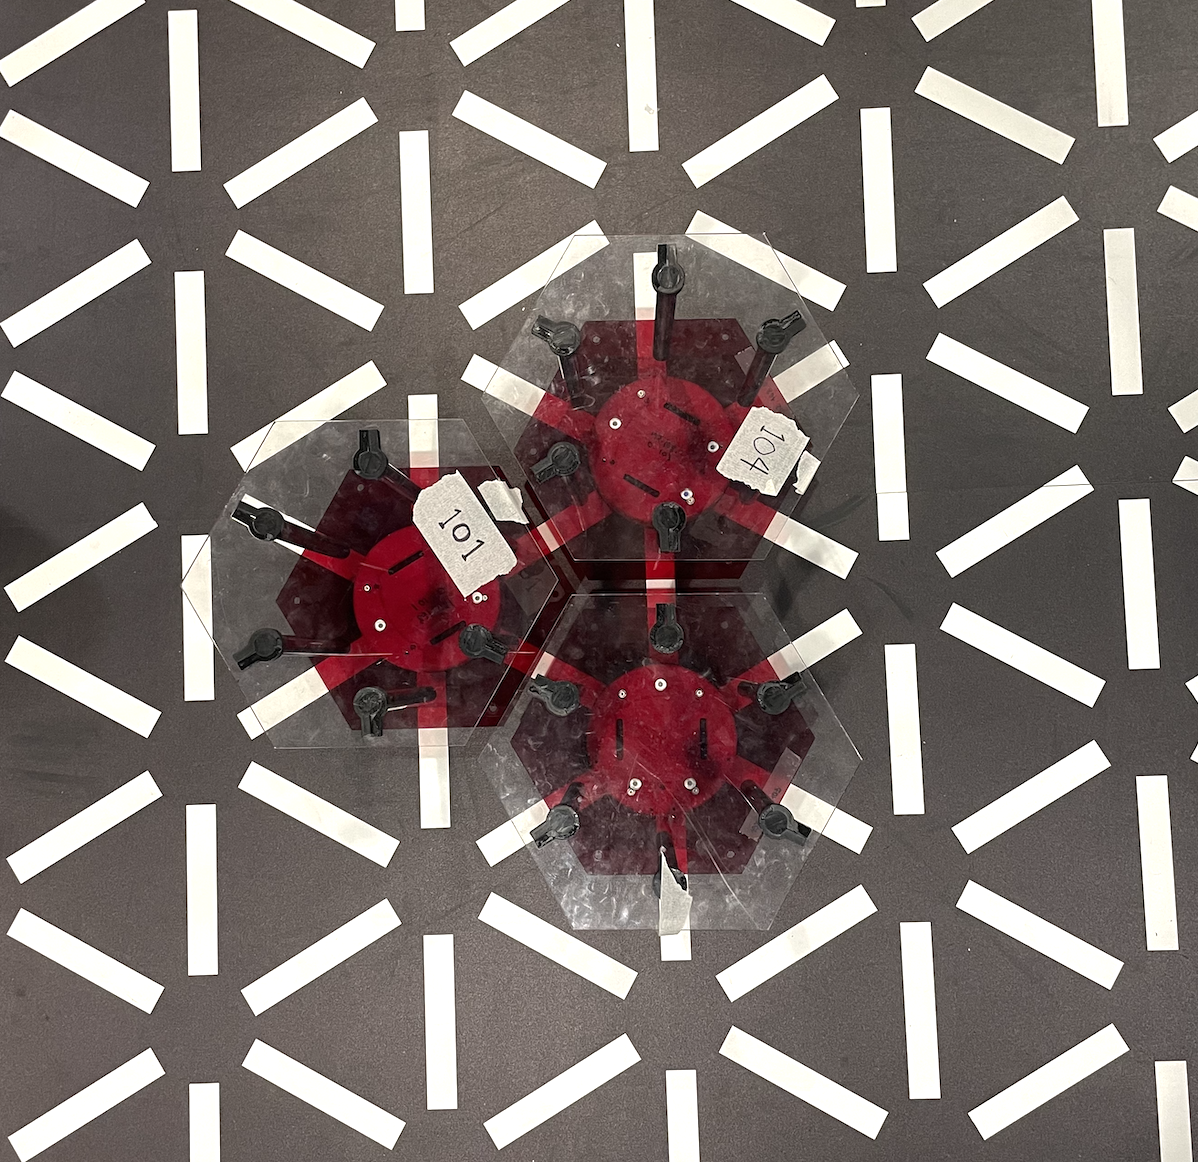
\includegraphics[scale=0.35]{images/irl_maze.png}
    \caption{This figure shows a top down view of one of the configurations of the honeycomb maze where there a hexagonal grid where the hexagonal robots are placed on top. Upon one of these platforms the animal would be placed on the hexagons and would choose which platform to move to.}
    \label{fig:picture_of_maze}
\end{figure}

There are three platforms on the hexagon space and one has the animal placed on it. They is all placed in a room with the hexagonal grid marking on the floor, representing the maze that the animal traverses.

The stated goal of the algorithm is as follows:
\begin{enumerate}
    \item(Fig. \ref{fig:example_algorithm} Panel A) The animal is placed on a platform robot with is consecutive to two other platforms. It can either chose to move to one platform or the other. This is entirely the mouse's decision (shown in Fig. \ref{fig:example_algorithm} panel B).
    \item After the mouse has made this choice, it must move the remaining platforms \textit{without} the animal on it so they are newly positioned next to the new platform with the animal on it (as shown in fig. \ref{fig:example_algorithm} panel C).
    \item This cycle will continue until the mouse has reach the goal required by the experimenter.
\end{enumerate}

An example of what the function of the algorithm's function is, is shown in Figure \ref{fig:example_algorithm}. Note that in this figure the arrangements of the hexagons around the central green platform are examples only. They can be placed anywhere around the central green platform as shown in panel C of Figure \ref{fig:example_algorithm}.

\begin{figure}[H]
    \centering
    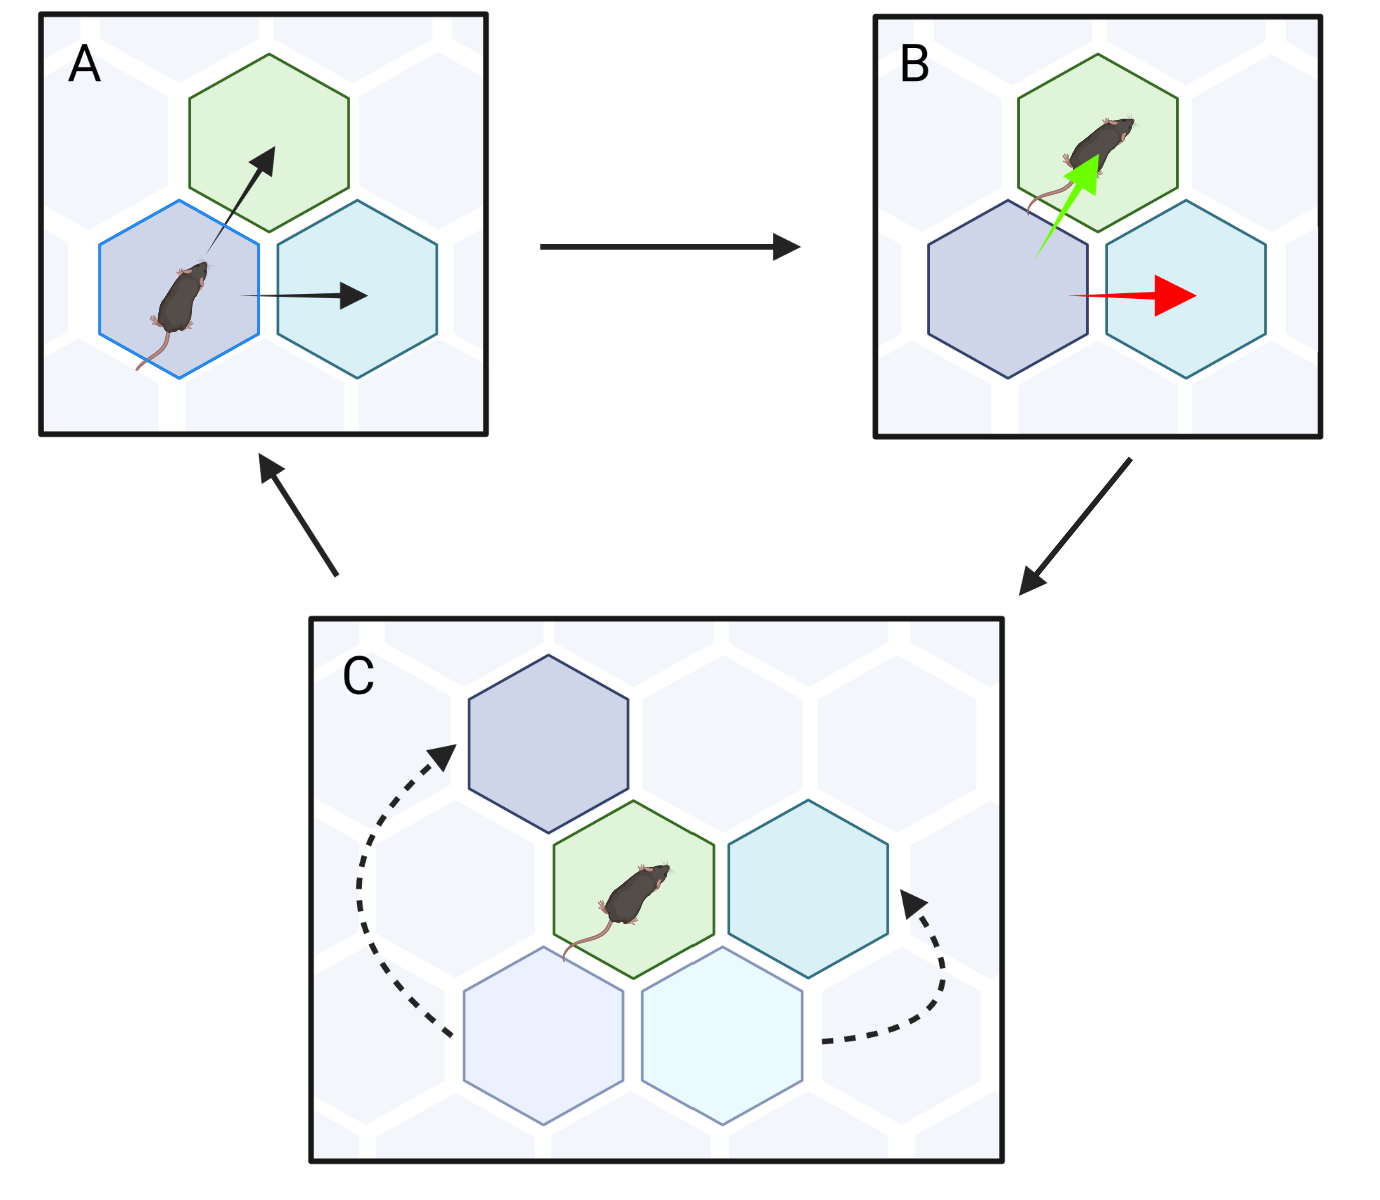
\includegraphics[scale=0.6]{images/example_algorithm.png}
    \caption{This figure shows the an overview of the function of the algorithm that has been developed for the making of the Honeycomb Maze. \textbf{Panel A} shows the animal on the dark blue platform where it can choose to move to either the green or the light blue platform. \textbf{Panel B} shows that the animal has chose the green platform to move to, and the light blue platform has \textit{not} been chosen. \textbf{Panel C} shows the function of the algorithm developed; it moves the dark blue and the light blue platforms respectively to their new places around the hexagonal platform with the animal on it so that the mouse can choose which platform it will move to again.}
    \label{fig:example_algorithm}
\end{figure}


\subsection{Hexagonal Grid and \textit{Khepera IV} Robots}
% Section about the grid upon which the robots are placed

On the floor of the experimentation room a hexagonal grid is printed (as shown in Fig. \ref{fig:hexgrid_with_numbers}). There are light grey lines on a dark black background; these lighter lines are detected by infra-red (IR) sensors on the bottom of the robots \ref{fig:robot} and used to know how far they have rotated or translated across the grid.

\begin{figure}[h]
    \centering
    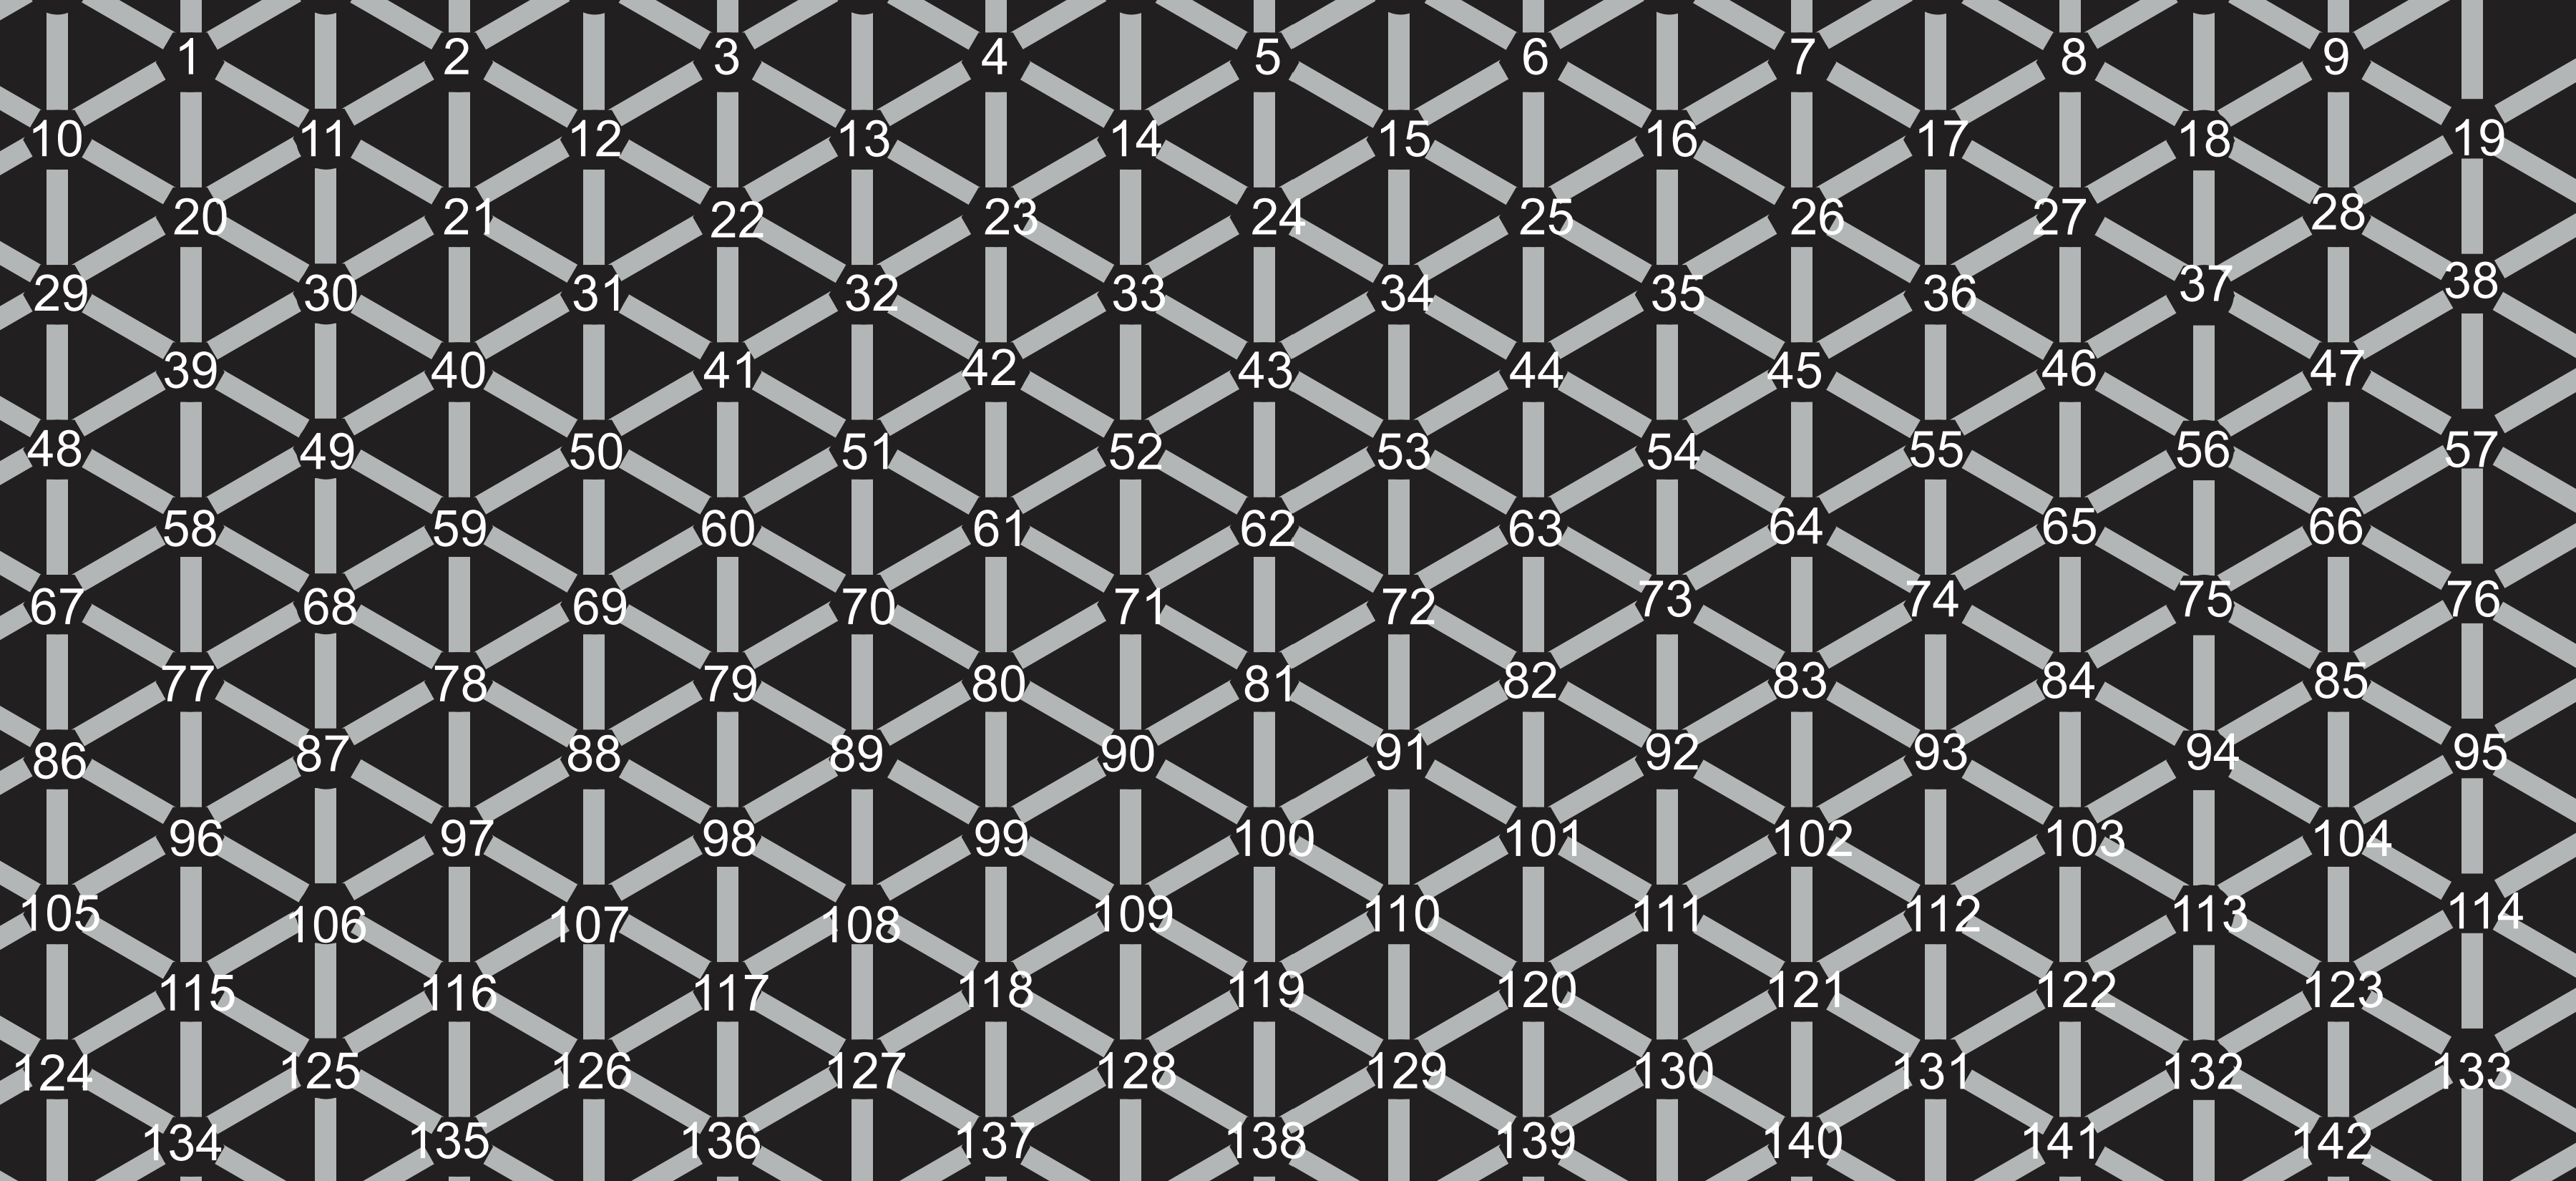
\includegraphics[scale = 0.3]{images/hexgrid_with_numbers.png}
    \caption{This shows the mat on the floor of the experimentation room which, upon which, the line following robots will navigate. The black and light grey lines can be detected by the line following robots' IR sensors.}
    \label{fig:hexgrid_with_numbers}
\end{figure}


% Section about the Khepera IV robot, their design and hence the limitations

The robots used in this maze are the \textit{Khepera IV} robots (see Fig. \ref{fig:robot}). On their bottom surface, they have IR sensors allowing them to detect when they have passed over a light grey line. 
This allows to them to keep track of the number of rotations they have made in place or the number of translations they have made. This allows reliable navigation the around the hexagonal space they inhabit.

Due to the parallel arrangement of the wheels on the underside of the robots, they are only able to move forwards and backwards or turn in place. In order to alter the direction of travel, the robots must first rotate \textit{and then} translate.

Therefore, whenever the platform robot wants to move to the out of its current direction of travel, it must first rotate to its desired direction of travel and then translate forwards.

\begin{figure}[h]
    \centering
    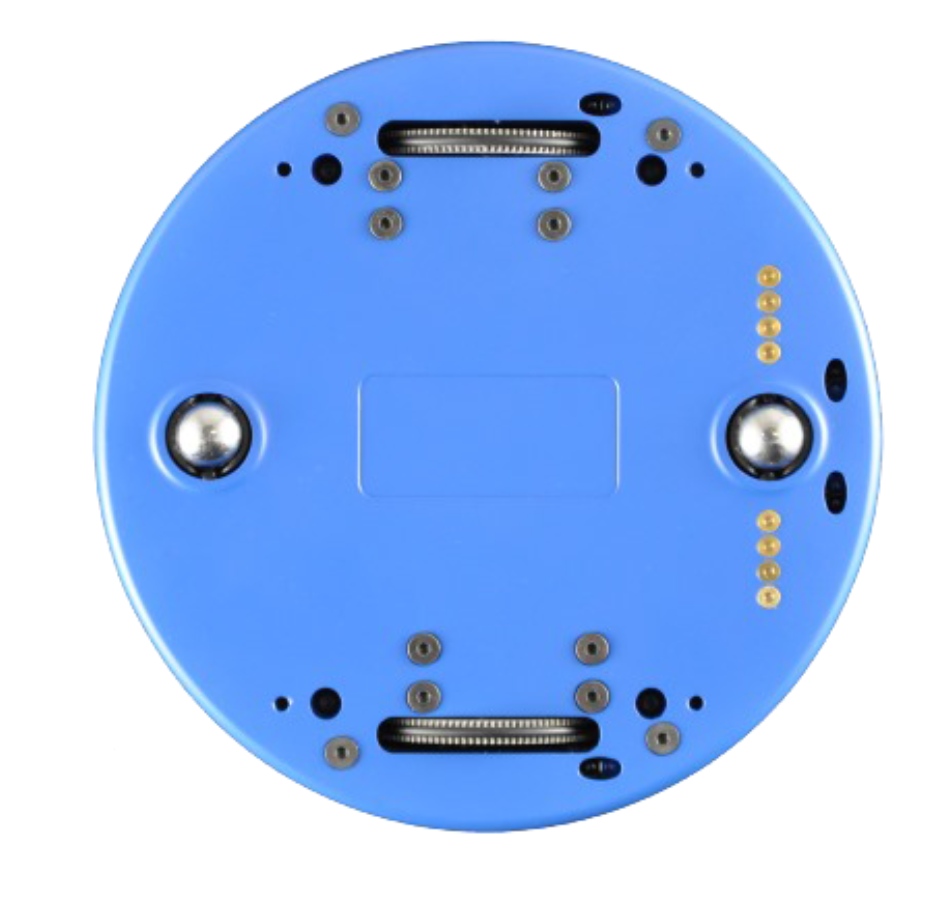
\includegraphics[scale = 0.5]{images/khepera_IV_robot.png}
    \caption{Shown is the underneath of the \textit{Khepera IV} robot. Note the presence of the 2 parralel wheels of the robot. This leads to signicant movement limitations of the \textit{Khepera IV} robots which must be addressed in the development of the program to control the Dynamic Honeycomb Maze.}
    \label{fig:robot}
\end{figure}

\subsection{Platforms}

%Section about the design of the platforms of the robot and the limitations that come with it
Due to the hexagonally tiled space, shown in Figure \ref{fig:collision}, consecutive tiles cannot rotate next to each other, otherwise they will collide.

\subsection{Summary of limitations of the line following robot and its platform.} 

Below are the intrinsic design constraints that the program will have to overcome for a successful Honeycomb Maze to be developed:
\begin{tcolorbox}
\begin{enumerate}
\item Two hexagonal platform \textit{that are adjacent} are unable to rotate without colliding. To avoid this, a robot cannot be adjacent to another robot when they rotate (see Fig \ref{fig:collision} for example collision).
\item Due to the parallel wheels of the robot, they have a sense of polarity, meaning they can not change direction without rotating first.
\end{enumerate}
\end{tcolorbox}
This results in a limited range of movement of the platforms when they are consecutive to each other and are in fact only able to move without restriction when they are not consecutive to any other platform robots.

\subsection{Development Environment}

%Justify the use of python 
The development of this package has been done in Python 3. This allows the integration of other libraries for simplifying the program.
The program developed, will return a list of commands that are given to the \textit{Khepera IV}. These will be executed by the  \textit{Khepera IV} to move around the hexagonal grid upon which it is placed.


% \subsection{Network of Integration}

% Explain how the python code will interact with the robots directly.

As the aim of this dissertation is to develop a tool for investigating the behaviour of mouse models, is it also an important aim for the program to be structured such a way that modifications to the code to add new behaviour in the future are possible



\pagebreak

%Implementation
\section{Implementation of Dynamic Honeycomb Maze}

The design of this maze has three basic interacting units.
They are:
\begin{enumerate}
    \item The \textbf{\textit{Animal}}, which makes a decision about which platform it would like to move to.
    \item The \textbf{\textit{Robot}s}, which  move around grid as required to give the animal the choices about where it would like to move to next.
    \item The \textbf{\textit{Maze}}, which is the set of all points in the grid within which the robots can navigate around in.
\end{enumerate}
As such the program has been structured into these three basic parts where the relevant functions are placed into the relevant classes.

\subsubsection{\textit{Inner Ring}, \textit{Outer Ring} and \textit{Relative Position}}

% The idea the platforms have to compute their distance in correlation to each other, not based on their absolute distance in the maze from each other

% Because of how often these ideas are used in the code, the inner ring, outer ring and relative position are used introduced at the start of the program

% Because of the importance of these two ideas in the development of this algorithm these two ideas have been introduced before the explanation of where they are used in the algorithm.

The movement of the robots occur in relation to each-other, for example 'a movement \textit{away} from another robot' or '\textit{around} each other'. As such  these relative heuristics are developed for computing the robots' place in relation to each-other and are used in many parts of the program to compute moves.

\paragraph{Inner and Outer Ring}

The \textit{inner ring} is the set of 6 hexagonal tiles that are consecutive to one central tile. These are the orange tiles in Fig \ref{fig:inner_ring}.
The \textit{outer ring} are the set of 12 tiles that are all exactly 2 moves away from the central tile (blue tiles in Fig \ref{fig:inner_ring})
Often the inner and outer ring will be computed from the animal robot position (as shown in Fig \ref{fig:inner_ring}). See function \ref{function:def_inner_ring} for implementation.

\paragraph{Relative position}

Relative position acts as a mapping of all the six hexagonal points on the inner ring to point on the outer ring where relative position is defined. This come in useful when setting path-finding targets in Section \ref{section:pathfinding_targets}.
See function \ref{function:def_relative_position} for implementation. t


\begin{figure}[H]
    \centering
    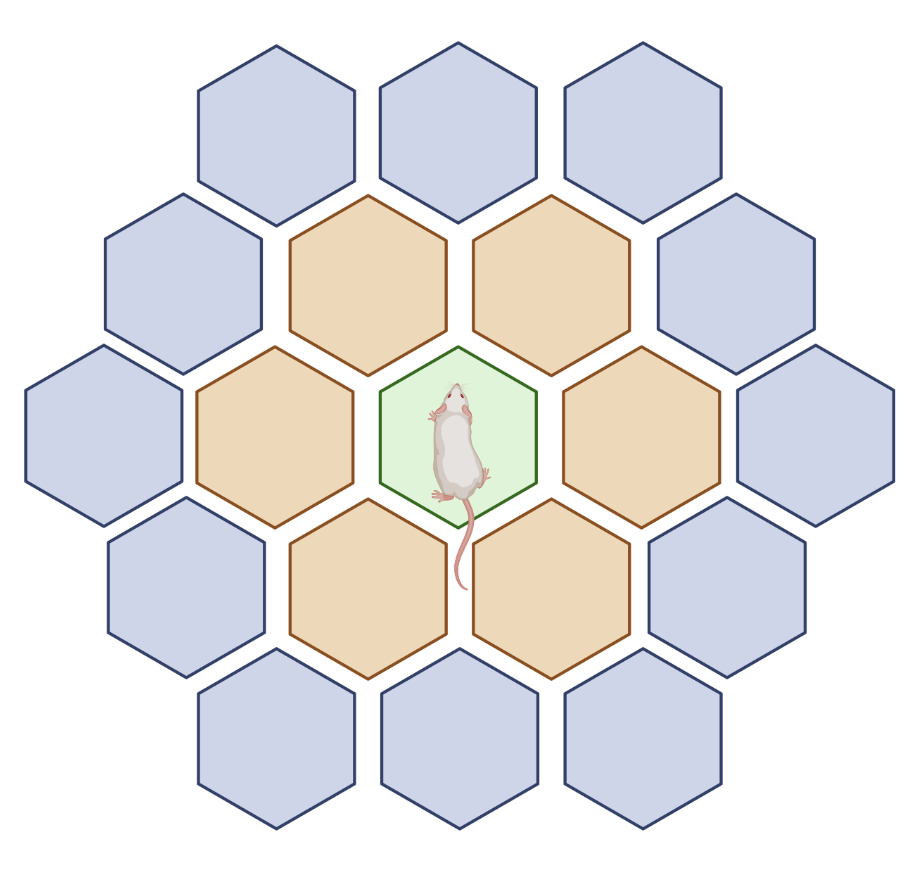
\includegraphics[scale = 0.5 ]{images/outer_rings.png}
    % 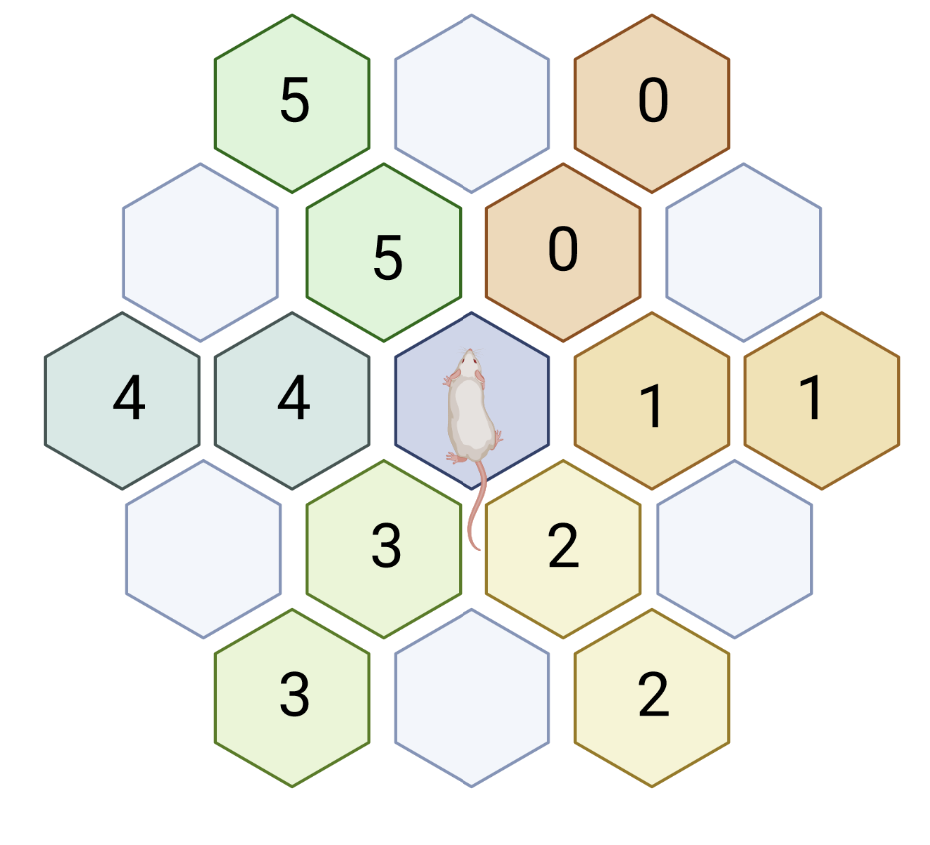
\includegraphics[scale = 0.50]{images/relative_position.png}
    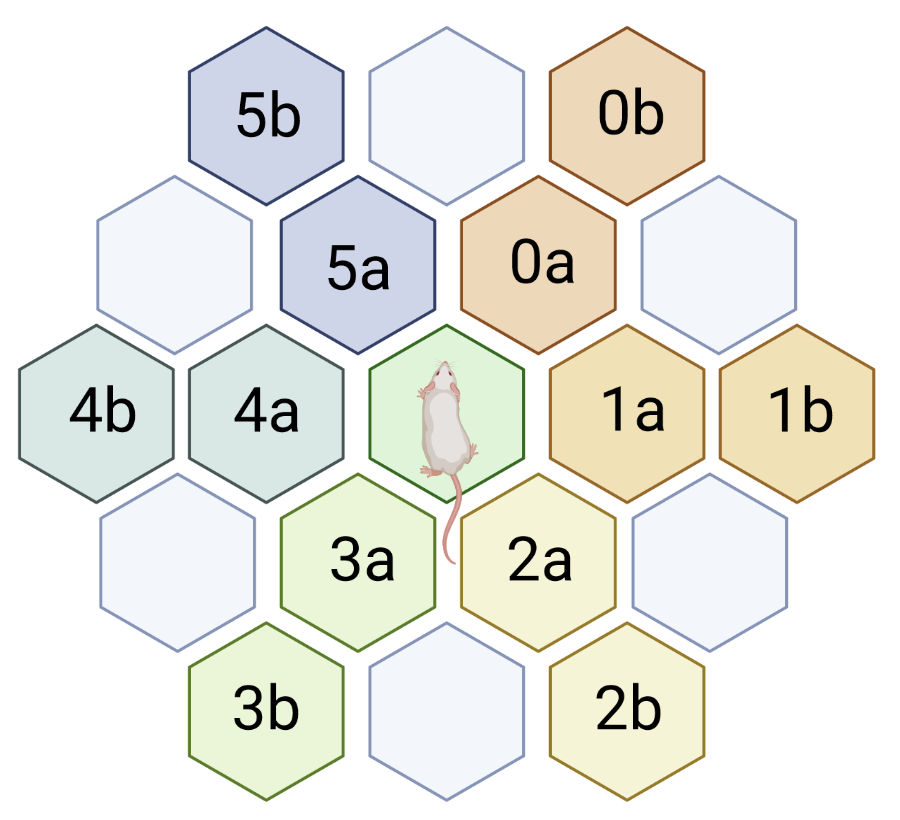
\includegraphics[scale = 0.50]{images/relative_position_mapped.png}
    \caption{This figure shows two important concepts that have been developed: 1. LHS: Inner (\textit{Orange}) and Outer Ring (\textit{Dark Blue}). 2. RHS: Relative Position}
    \label{fig:inner_ring}
\end{figure}


\subsection{\textit{Maze} Class}


This is the class which handles the area which the robot platforms move around.
It is important, for handling the boundaries of the maze, defining where robots are allowed to move without letting the path finding algorithm running out of space to complete its moves.

\subsubsection{Coordinate system}

Despite the surface on which the platform move around on being a 2D space, for the task as hand it is can be more intuitive to use a 3D coordinate system to encode the space traversed by the robots. This is because there are six directions the platforms can move out of any point in the grid. This can be thought of as three dimensions (where there is a backwards and forwards direction for each of the three dimensions). These are: the $North-East$ direction, the $East-West$ direction and the $North-West$ direction.
For this program, it has been decided that movement in the $North-East$ direction has been considered to be the positive $y$ direction, $East-West$ direction to be the positive $z$ direction and the $North-West$ direction to be considered positive $x$ direction and vis versa.

The mathematical embedding of this space is a slice through 3D coordinate system, taken through a diagonal of a cube and what is left is a hexagonal shape (exemplified by Fig. \ref{fig:hexagona_slice_through_cube}), more specifically the plane:
$$x + y + z = 0$$
 
This forms a hexagonally tiled surface can be used to as the plane on which out robots move through.

Based on theses rules the following figure shows the coordinate space that has been used. 
\begin{figure}[h]
    \centering
    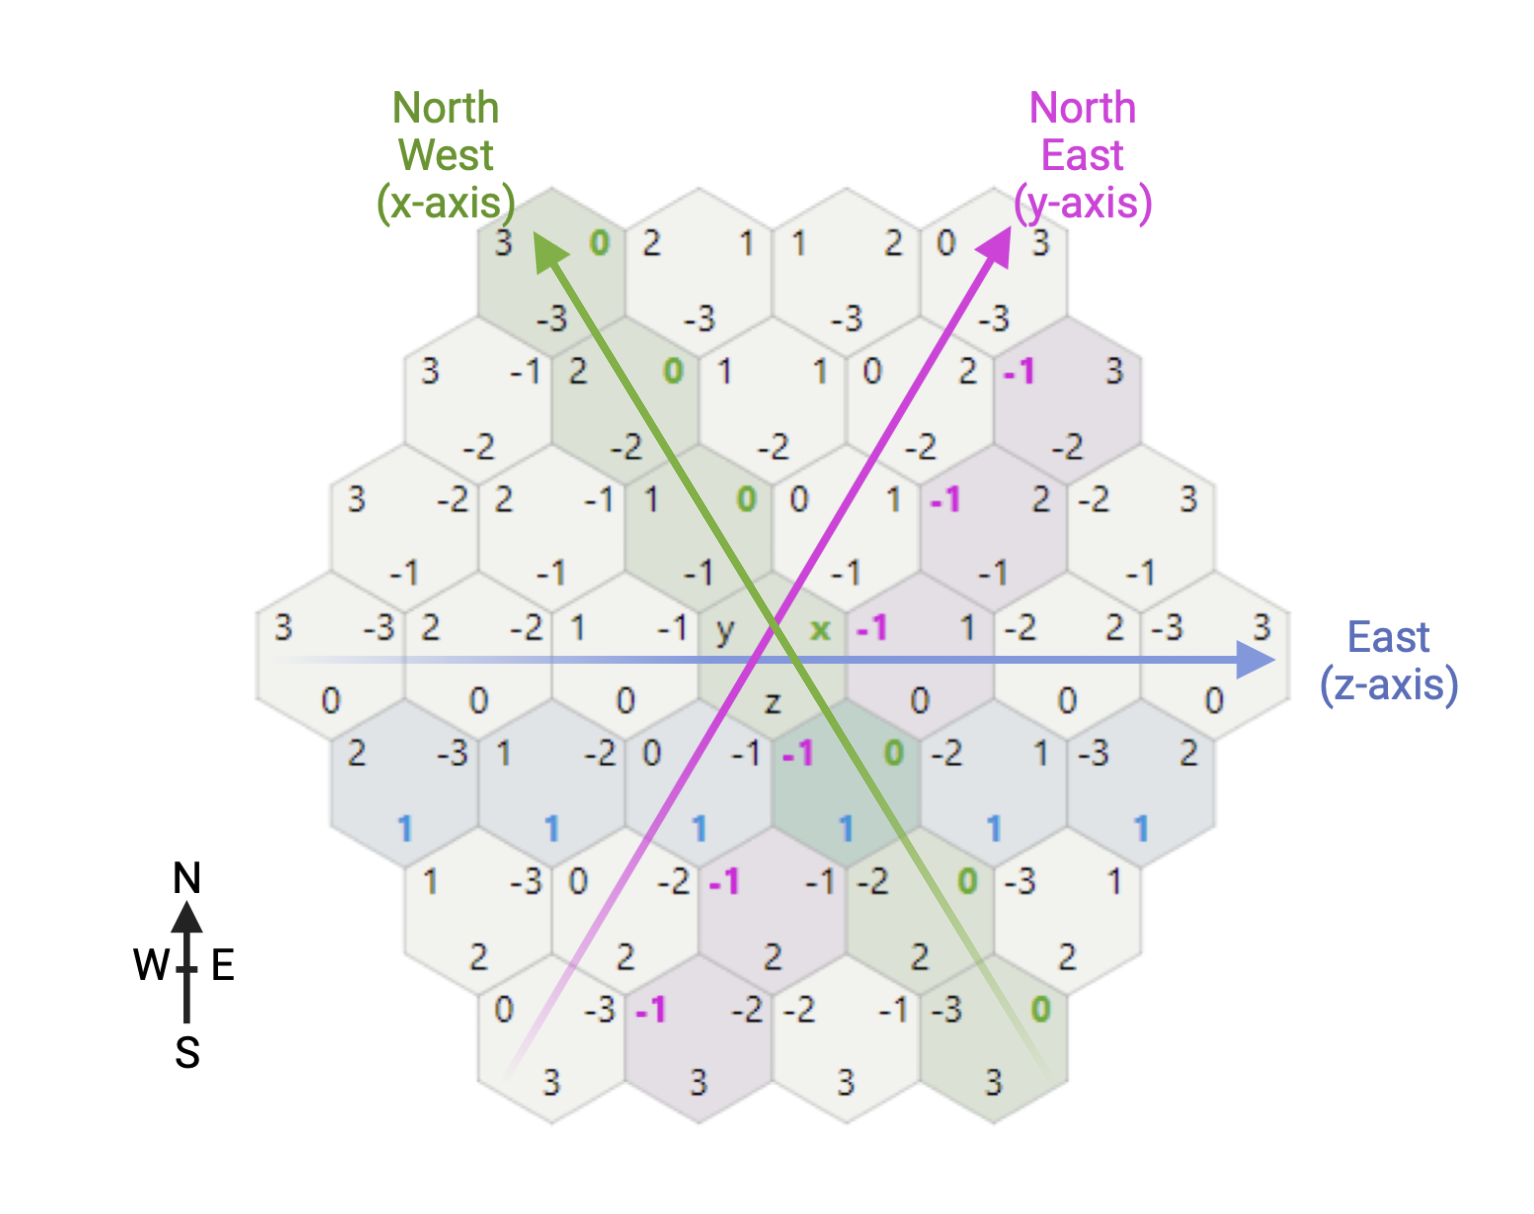
\includegraphics[scale=0.35]{images/hexagon_coordinates_adapted.png}
    \caption{The coordinate system used to encode the 2 dimensional space with a 3D coordinate system. The axis have been defined $North-West$ as $x$, $North-East$ as  $y$ and $East-West$ as $z$. This figure has been adapted from Red Blob Games \cite{patel_2021}}.
    \label{Hexagonal grid coordinates}
\end{figure}

Due to the novel coordinate system being used, a function has been defined in the \textit{Robot Class} which moves the robot around the coordinate space in a way that ensures the robots position remains valid (see Function \ref{function:move_around_hex_grid}).

\pagebreak
\subsection{\textit{Robot} Class}

This is the class which deals with the movement of the robot around the maze in which it is places. Notably, this includes the path-finding algorithm for the robots to move from the initial position to their final position and all the supporting functions required.

\subsubsection{Overview of the whole path-finding process}

The order of the overall algorithm requires the following steps:
\begin{tcolorbox}
\begin{enumerate}
    \item Deciding the order by which the platforms move so that no collisions take place. (See  Section \ref{section:order_of_operations})
    \item Movement of the platforms away from the animal robot so it can move freely without collision. (See Section \ref{section:pre_pathfinding})
    \item Path-finding around the board to their path-finding targets using the Dijsktra Path-finding Algorithm. (See Section \ref{section:pathfinding})
    \item Moving into the inner ring of the animal robot so they are in the new positions so that they are consecutive to the animal allowing the animal can make another decision to choose another platform around the maze. (See Section \ref{section:post_path_finding})
\end{enumerate}
\end{tcolorbox}


\begin{figure}[h]
    \centering
    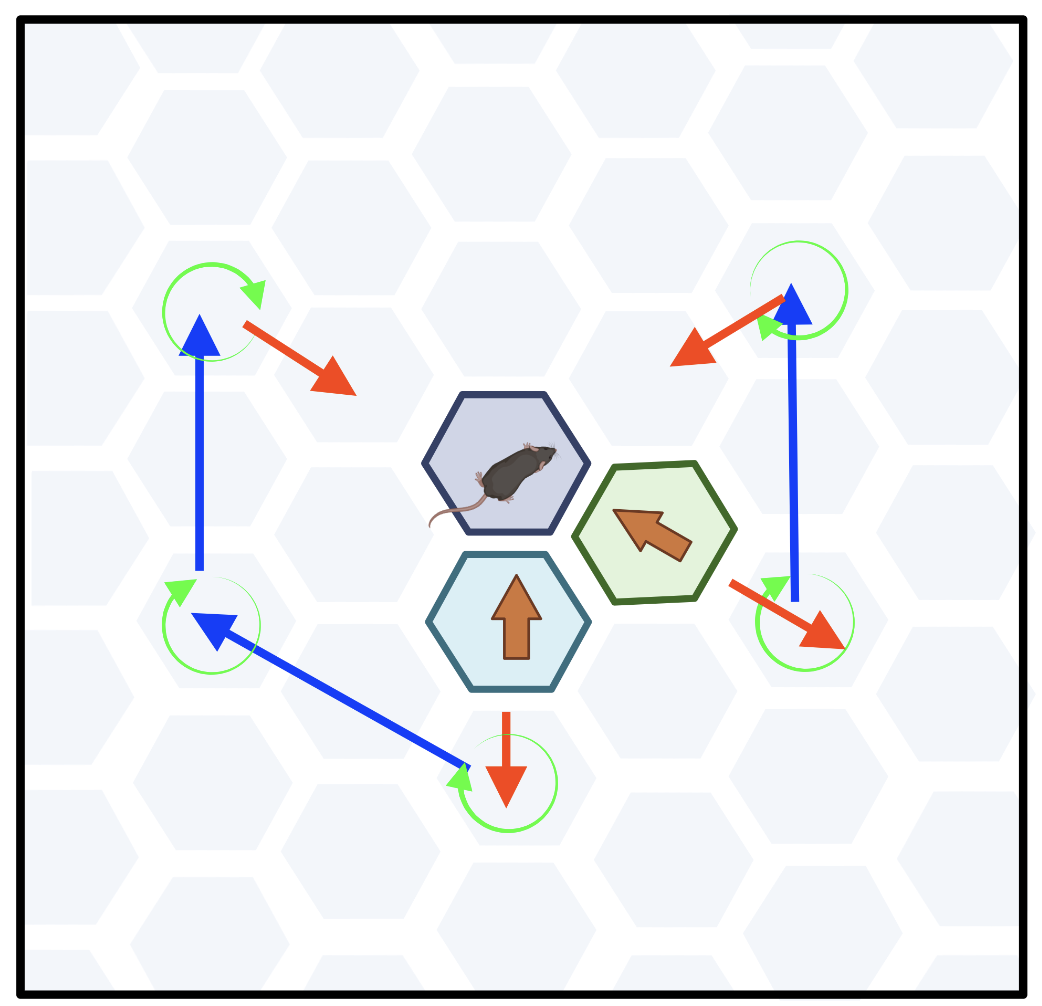
\includegraphics[scale=0.4]{images/overview_of_algorithm.png}
    \caption{This shows an example of the overall movement that would occur when moving the robot around}
    \label{fig:overview_of_algorithm}
\end{figure}

\subsubsection{Order of movement of the platforms}
\label{section:order_of_operations}
Here we discuss the order of operations for that the two moving platforms must take as to not collide with each other. There must be no collisions for all possible pairs of positions of the non animal robots around the animal robot.

From Fig \ref{fig:post_decision_states} (and panel C from Fig \ref{fig:control_flow_diagram}) we see that the platform which the animal did not choose to move on to, must be the first platform to move backwards away from the robot which used to have the animal on it. If this occurs, the platform is never consecutive to the other two platforms meaning it has free range of movement to start the path-finding phase.

After this has occured, the robot animal on it and the robot which used to have the animal on it left consecutive to each other (so there is limited range of movement).

The robot, with no animal on it, that is left consecutive to the (current) animal robot must always step back into the outer ring of the (current) animal robot. Similarly, this allows the robot free range of movement as it is not consecutive to any other robots.

These two observations imply: (1) that the robot not selected must always move first, and (2) the robot that used to be the animal robot must always move second.

It follows from this that the concept of 'animal robot', 'non-animal robot' and 'non-non-animal robot' can be developed.
\begin{tcolorbox}
They are defined in the following way:
\begin{itemize}
    \item \textbf{'Animal Robot' (AR)} is the platform robot that the animal has choose to move to. This will always be \textbf{stationary} during the path-finding method.
    \item \textbf{'Non-animal Robot'(NAR)} is the platform robot that the animal has come from. This will always be the \textbf{second} robot to move in the path-finding method.
    \item \textbf{'Non-non-animal robot' (NNAR)} is the platform robot that the animal has not chose from the two choices. This will always be the \textbf{first} robot to move for the path-finding method.
\end{itemize}
\begin{center}
\textit{From now, the above notation will be used}
\end{center}
\end{tcolorbox}



Associated with this is the table for reassigning the robots' state, based on their previous state and new state which is shows in Table \ref{table:change_states_of_robot}).

Using this framework for choosing the order in which the moves must take place, it can be shown that the NNAR must always move first to prevent the colliding of platform robots as they are consecutive. 
This prevents there ever being arrangements of robots where the order of operations has to be calculated due to the arrangement of the direction of the robots.

\subsubsection{Pre-Pathfinding Phase}
\label{section:pre_pathfinding}

Recall: the animal will be given a decision about which platform to move to. Once this has occurred, the maze will be left with the configurations shown in Figure \ref{fig:post_decision_states} and appendix Figure  \ref{fig:all_post_decision_states}.



\begin{figure}[h]
    \centering
    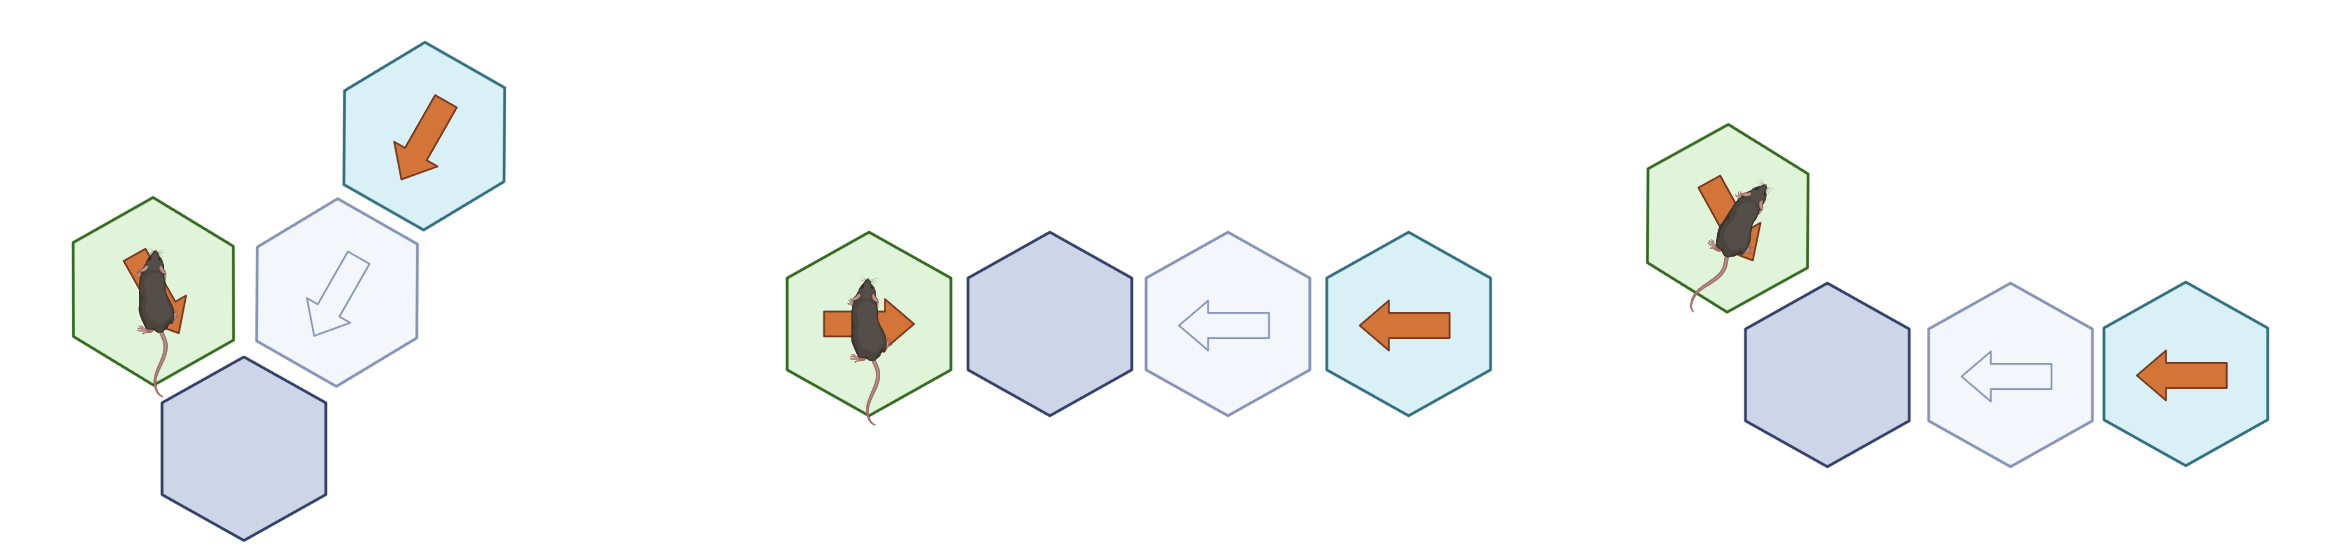
\includegraphics[scale = 0.5]{images/post_decision_state.png}
    \caption{This shows all possible arrangements of the three robots just after the animal has made a decision about which platform to stand on. In this case, the animal started on the blue platform as chose the green platform to stand on afterwards. \\ This demonstrates that the 'non-non-animal robot' must always step one step backwards from the other two robots to makes sure there are no other robots that are consecutive to it before it starts pathfinded to the outer ring position of the relative position of the path-finding end point.\\ \textbf{Note:} The \textit{dark blue} hexagon is the \textit{Non-animal robot (NAR)}, the \textit{green} hexagon is the \textit{Animal Robot (AR)} and the outlined hexagon is the \textit{Non-non-animal Robot (NNAR)}}
    \label{fig:post_decision_states}
\end{figure}

The strategies that are required for the \textit{Non-animal robot} and the \textit{Non-non Animal robot} are different and hence are handled differently. 

\paragraph{Non-non Animal Robot (NNAR)}

As demonstrated in Fig. \ref{fig:post_decision_states}, the NNAR must always move backwards away from the NAR. This is because this move will ensure that the NNAR is always not consecutive to any of the other robots in the system and hence free to move around.

\paragraph{Non-Animal Robot (NAR)}

Demonstrated in Panel D and E in Fig \ref{fig:control_flow_diagram}, the NAR must always move to the outer ring of AR, without turning. (Note: that this is sometime a step backwards and sometime a step forwards, depending on the rotation of the AR at the time.)

\begin{figure}[h]
    \centering
    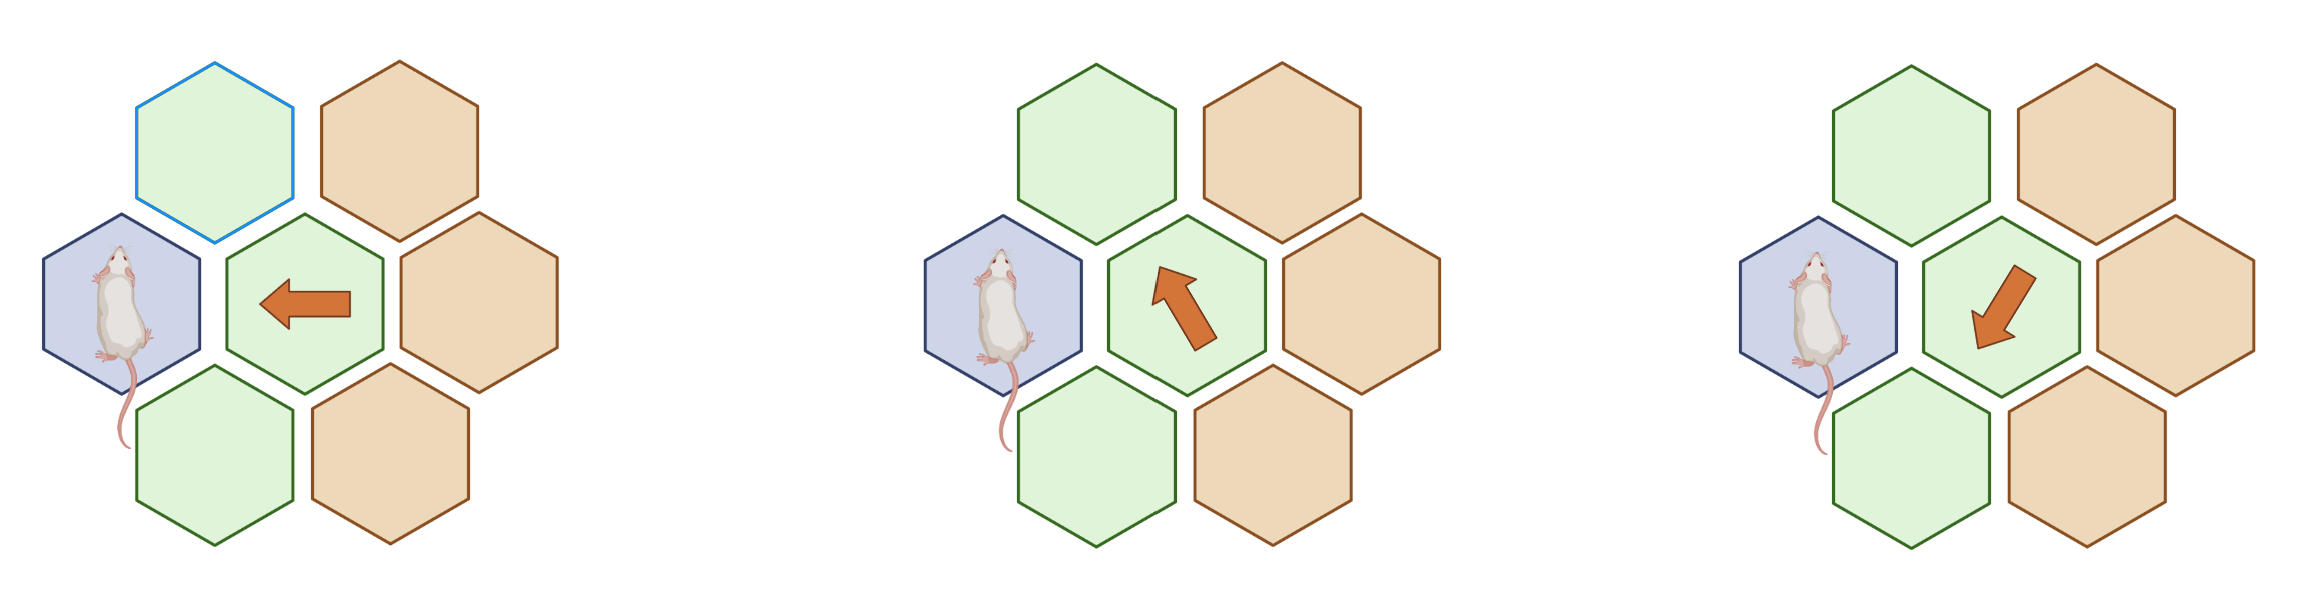
\includegraphics[scale = 0.5]{images/move_to_outer_ring.png}
    \caption{This figure demonstrates that whatever the position of the 'non-animal robot', it must step into the outer ring of the new 'animal robot'. This either means stepping forward once or backwards once, depending on what which was forward is each each of these arrangement. Importantly, note that is always possible for the 'non-non-animal robot' to move the outer ring.}
    \label{fig:nnar_move_to_outer_ring}
\end{figure}

\begin{tcolorbox}
Therefore, in the pre-pathfinding phase of the algorithm:
\begin{enumerate}
    \item NNAR will always move (first) way from the NAR.
    \item NAR will always move (second) into the outer ring of the AR.
\end{enumerate}
\end{tcolorbox}

\subsubsection{Pathfinding Phase}
\label{section:pathfinding}

\paragraph{Justification of \textit{networkx} approach} 

A general path-finding algorithm was implemented, instead of a hard-coded' solution more specific to the task at hand, because a general path-finding algorithm allows a more versatile version of the program handling more combinations of robot positions without the algorithm failing to find a valid path.

To prevent having write source code for a general path finding algorithm, a python library, able to find the shortest path between two points on a network, called \textit{networkx} \cite{networkx} was used instead. This requires the path finding problem presented to be converted into a graph which the library can handle.

The most advanced path-finding algorithm \textif{networkx} supports is the \textit{Dijkstra} path-finding algorithm \cite{dijkstra1959pathfinding}. Though it is not as efficient or versatile as other path-finding algorithms, such as the A*  path-finding algorithm \cite{A*_pathfinding} \cite{lit_review_pathfinding}, for the size and complexity of network that will be generated for the honeycomb maze, the Dijkstra path-finding algorithm will  suffice. Due to the computational time required to find the path being negliable compared with the time taken for the path found to be executed by the robots.

\paragraph{Implementation of \textit{networkx}}
From the hexagonal grid determined by the \textit{Maze} class, a triangular lattice network of the correct size is generated. This encodes all positions (coordinates) that are possible for the robots are able to move to in the room. A triangular lattice is used as this network connects all nodes (not on the boundary of the grid) to six consecutive nodes, which is the same as the number of adjacent movements possible from each point on the grid.


After the whole movement network was generated, a modified version of the movement network was generated: the \textit{temporary movement network (TMN)} with all moves that would cause collision being removed from the network. When a robot wants to move around the network the positions of the 'non-moving' robots were removed from the \textit{TMN} as well as the \textit{inner-ring} positions for these same robots - as these are the positions that would cause collisions if the robot was moved there.
The \textit{TMN} would be returned to the moving robot, where it would find its path from the \textit{path-finding source} to the \textit{path-finding target}.

\begin{figure}[h]
    \centering
    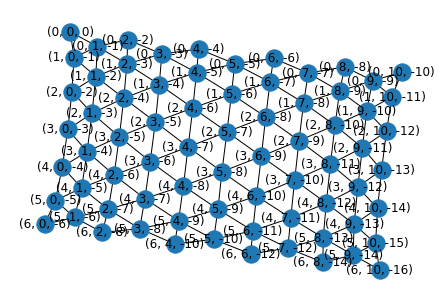
\includegraphics[scale = 0.3]{images/output.png}
    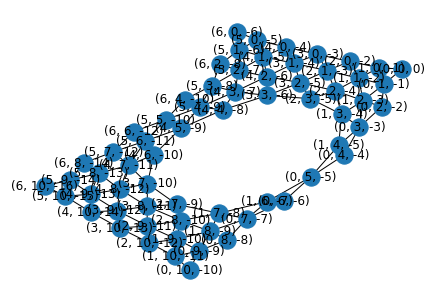
\includegraphics[scale = 0.3]{images/output2.png}
    \caption{This shows an example of the network generated by the \textit{networkx} library (LHS image), based on all the possible moves available in the maze. Once the network has been generated, the positions that are impossible to access by the moving robot are removed from the network (RHS image). From this, the shortest path from the \textit{path-finding source} to the \textit{pathf-inding target} will be found and a list of coordinates that describe the path will be generated and return to the robot. This figure has been generated by the \textit{networkx} package \cite{networkx}.}
    \label{fig:networkx_diagrams}
\end{figure}


\paragraph{Setting Path-finding Targets}
\label{section:pathfinding_targets}

Since the actual source and target of the complete algorithm will always be in the inner ring of the 'non-moving' robots, they are removed from the \textit{TMN}.  As such, they can not be used as the path-finding source and target for the path-finding algorithm. 

Therefore, the source and target used, are corresponding outer ring positions of the actual source and target. They way these are calculated, corresponds to the mapping shown Fig \ref{fig:pathfinding_source_target_mapping} from the (blue) inner relative positions to the (pink) outer relative positions.

This allows the moving robot to get to the correct relative position of its target position, however instead of being in the inner ring, where it aims to be, it is in the outer ring.
% From Fig. \ref{fig:inner_ring}, it can be seen that to get to the inner ring for each relative position, the robot must reach the corresponding relative position on the outer ring and simply move one step towards the animal robot to reach its final position.

% This mapping of every position of the \textit{inner ring} to a position in the \textit{outer ring} has been called \textit{relative position} and can be calculated from the position of any given platform robot. See Table \ref{table:relative_position_truth_table} and Function \ref{function:def_relative_position} for its implementation.

% Based on the \textit{relative position} of the actual goal platform, the path-finding goal is generated by finding the \textit{outer ring} counterpart of the \textit{inner ring} with the same relative position. This is done so that once the robot reaches the outer ring relative position, a standard algorithm can be used to turn the NAR or NNAR to the AR and then step forward (at the same time) to become adjacent to the robot at the same time (see Function \ref{function:move_to_inner_ring)}

\begin{figure}[h]
    \centering
    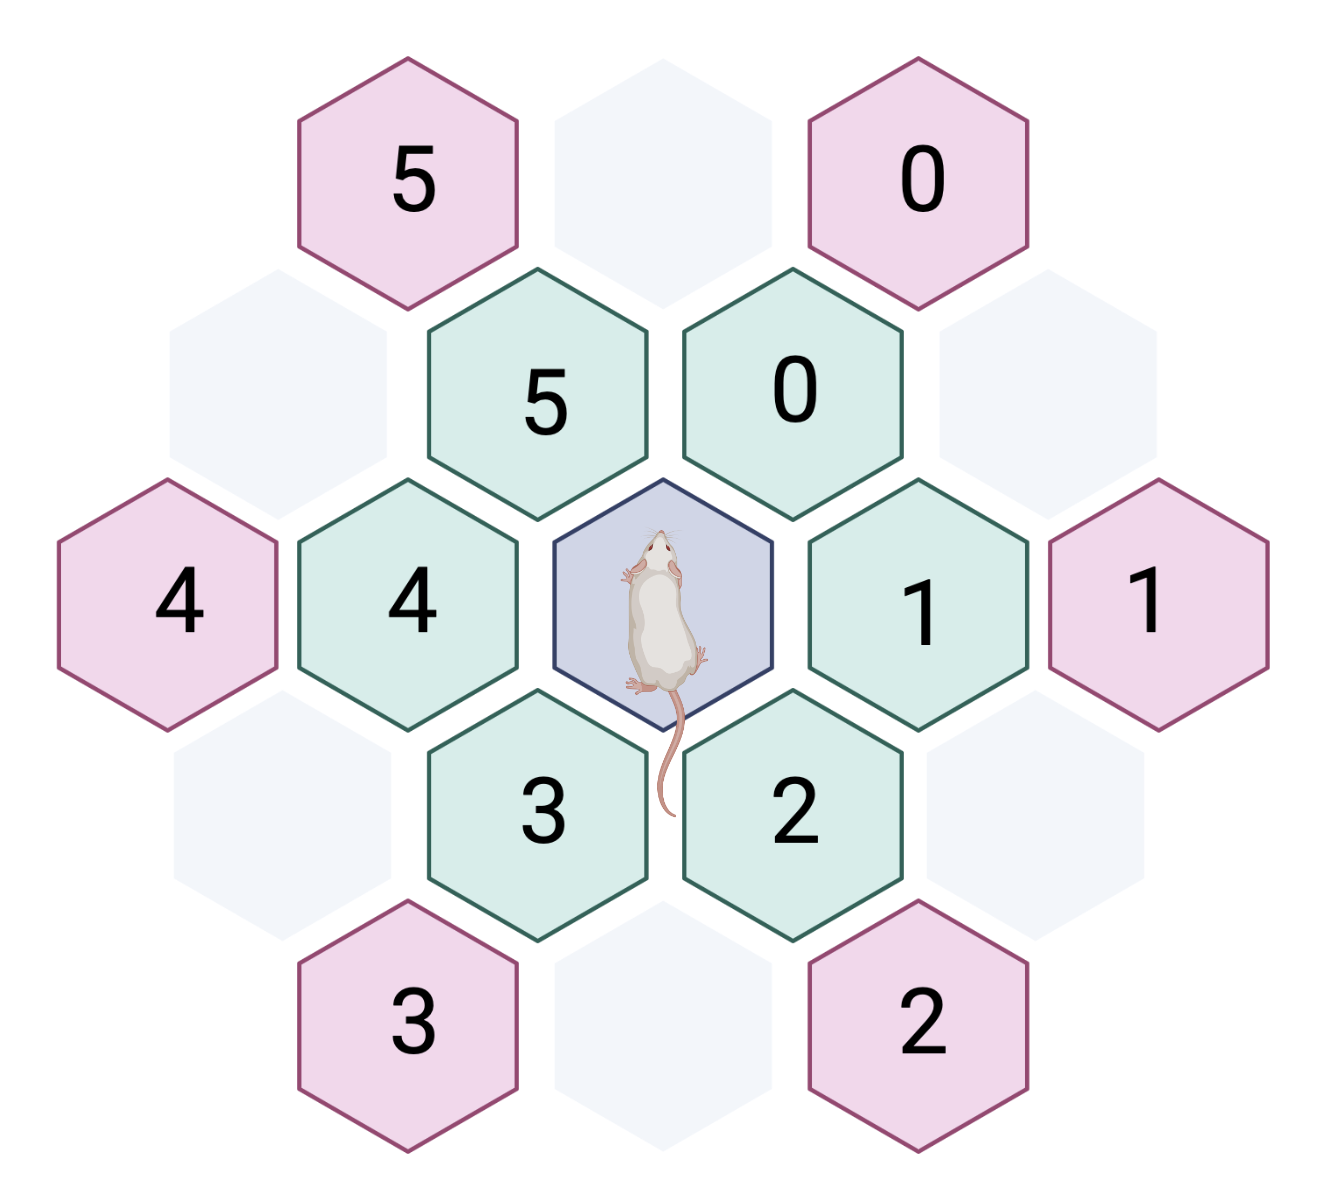
\includegraphics[scale=0.25]{images/pathfinding_source_target.png}
    \caption{This figure shows the mapping from the actual source (or target) of the pathfinding algorithm (in blue) to the 'pathfinding source' or 'pathfinding target'  (in pink). This is because \textit{networkx} will not be able to pathfind from a position in the network that is not present. As such, the pathfinding begins after the 'step back from the NAR' move takes place.}
    \label{fig:pathfinding_source_target_mapping}
\end{figure}

\subsubsection{Post-Path-finding Phase}
\label{section:post_path_finding}

As shown in Fig. \ref{fig:nnar_move_to_outer_ring}, after the animal has made its decision, the NNAR must move to the outer ring to make sure that it does not collide with the NAR when executing its path.

The NNAR, which moves first will wait until, the NAR has moved to its path-finding source. Once both of the moving robot (NAR and NNAR) have reached the end of their pathfinding phase, they will both be in the outer ring of their correct relative position. 
They must both move to from their outer ring position to their equivalent position in the inner ring. This is what occurs in the \textit{Post-Dijsktra Phase} of the algorithm. 

The NNAR will wait for the NAR to be in position. Once this has occurred, both NAR and NNAR will move from their \textit{outer ring} position to their corresponding \textit{inner ring} position, providing a choice for the animal to choose which platform it would like to move to.
This command will be executed at the same time for both robots. This makes sure the animal has the same amount of time to consider each platform, reducing bias to a particular platform.


\subsubsection{Moving to final position}

Once the robots has reached their path-finding target, it will be in the in the correct relative position of the required target, however it will be in the outer ring, not the inner ring (as required). Therefore, a move to the inner ring from the outer ring is all that is required to move to its correct position. (In Fig \ref{fig:pathfinding_source_target_mapping}, they will have to move from the (pink) outer ring to the corresponding position (blue) position in the inner ring.

% From combining the ideas from Figure \ref{fig:inner_ring}, it can be seen that the relative positions is a one to one mapping of the six positions on the inner ring to six positions on the outer ring. This becomes very useful because once a robot on on the outer ring position (where the relative position is defined), it can be used to move the robot from the inner ring to the outer ring in a standard way.

% Once the robot has got to the outer ring of the animal robot, where the relative position is defined, all that the robot has to do is to move from the outer ring to the inner ring whilst staying on the line of the same relative position.

% The non animal robot (or non-non animal robot) simply has to point towards the animal robot. Once it has done this, the animal robot simply has to step once forward. Then it will be consecutive to the animal robot. Once this has occurred the animal can make a decision about which robot platform it would like to move  towards.

Both the \textit{NAR} and \textit{NNAR} will be pointing towards to \textit{AR} when they step forward to get from the outer ring to the inner ring. This means they will \textit{always} be pointing towards the \textit{AR} in their final position. Therefore, the start positions shown in panel A of Fig \ref{fig:control_flow_diagram} are all the valid starting positions that the algorithm must handle.

\\ \\ 

This method of doing the final step in the algorithm means that the platforms can never reach an arrangement where it is hard to deal with their movement. This is because both the non-animal robot and the non-non animal robot will always point towards the animal robot (as is shown in panel A of Fig \ref{fig:control_flow_diagram}) and not be locked into an arrangement which requires a different order of operations that what was described in Section \ref{section:order_of_operations}. 

\pagebreak
\subsection{\textit{Animal} Class}

This class is defines the position of the animal, which must always be on one of the robot platforms. The \textit{animal} class is also used for to model the decision making that the animal made when testing the program.


\subsubsection{Animal class decision making}

Inside this class of the program, the animal robot can interface with \textit{deeplabcut} via simple function which takes the input of which platform the animal has choose to move to.

For testing the program, a simple random decision is made between the two possible choices of platform to move to for testing purposed
\pagebreak
%Results

\section{Results}

\pagebreak

% Discussion
\section{Discussion and Further Work}

\paragraph{Summary of Results}

The program is able to perform the task required by the design brief (see section \ref{section:design_brief})

\paragraph{Impact of the program}

Since this program is written in python, it allows easy integration with computer vision software such as \textit{deeplabcut} \cite{dlc}. This would allow the maze interaction to be automated.

A functioning version of this program has been uploaded to \href{https://github.com/casualcoffeeaddict/Honeycomb-Maze}{GitHub}. This means that for relatively little financial cost to the investigator, it would be possible for tool to be developed in many neuroscience laboratories investigating animal models of spatial cognition. This would be mean that it could be used more widely than just very well funded laboratories.
This would allow this tool to be used more widely in laboratories investigating spatial memory.  

\paragraph{Object oriented structure and expansion}

Because of the structure of the object oritented struture of the code (the object oriented structure to the code), it will be easier to modify and reuse to code to add features that are required in the further development of the honeycomb maze. 

An example of this could include a more efficient algorithm for setting the path-finding targets, which could easily be added to the program as the structure for setting path finding targets already exists.

New features can easily be added to the program. This is because it has been written in a modular and readable was according to the 'SOLID' framework for writing object oriented programs \cite{SOLID_book}.



\paragraph{Hard-coded steps in the implementation} In the overall algorithm, there were steps that were manually coded in that the robots must always perform under this version of the algorithm. These steps were namely the 'stepping back from the non animal robot' and 'stepping into the outer ring of the animal robot' in the start of the algorithm and the 'step into inner ring' at the end of the algorithm.

Due to the presence of these steps, the algorithm is not completely general, where for an increased number of platforms in the maze, the algorithm will still work. 

This is an area of improvement for the work, where the implementation for three moving platforms, for example, could be achieved.

Despite this, the algorithm in its current state is able to handle all the cases of movement that are required of it (except in cases where the animal robot is close to the corner of the area of the maze).

\paragraph{Function for deciding order of operations}

For a three agent system, it is possible to exhaustively manually search through the possible arrangement of the robots and hence workout the correct order of operations. However, in the case where there are most that three robots in the system, it could not be obvious what the correct order would be. It would be possible to write a function that calculates the correct order of operations for any number (and any position) of robots. This, however, would be a challenging task.

\paragraph{Assignment of Path-finding Targets}

For the development of a more efficient path-finding algorithm, that will have less steps between for the robots to take (on average), requires a more complex layer of logic that should be added to the program.

This would require the computation of all the possible targets from all the sources for each robot. From this the setting of path-finding targets so that average number of steps for each robot is as close to the mean of the selected choices. This would set the values so there are not extreme values for the path-finding (hence one robot does not have a very large number of steps to make compared with a very small number of steps to take for another robot so the the time for which any robot in the system remains still is reduced, so the robot time is not wasted waiting for other robots to move to their - far-away - targets.





% The steps required to do this would take the following algorithm:
% \label{function:move_around_hex_grid}
% \begin{algorithm}
% \caption{Better function for setting path-finding targets}
%  \begin{algorithmic}
%  \REQUIRE Robot List 
%     \FOR{Each Robot}
%         \FOR{Each Path-finding Target}
%             \STATE Find length of path
%             \STATE Add this the corresponding position in a matrix of path-length and robot
%         \ENDFOR
%     \ENDFOR
    
%     \FOR{Each Column in the matrix}
%         \STATE Find the average value for each of the columns
%         \STATE Find the variance of the columns
        
%     \ENDFOR
    
%     Return the column

%  \end{algorithmic}
% \end{algorithm}



\paragraph{Multi-Agent Path Finding (MAPF) Algorithms } 

The implementation of path-finding for both of the robots at once would be a way of increasing the speed of the algorithm as it would be able to compute paths for the both of the robots, from their path-finding source to goal at once. This would allow the execution of the commands to happen at once, reducing the time between animal decisions.

This is an area of research which has growing interest due to its use in multi-robot systems such as robotics-run run warehouses. There are implementations of this which are centralised such as the A* algorithm multi-agent systems \cite{DBLP:journals/corr/abs-2103-09979} or decentralised ways of organising behaviour such as the use of 'virtual pheromones' \cite{multi_agent_pathfinding_review} to communicate to many agents at once. 

The computational time required compute the best path, for the A* algorithm, can take significant computational run time ($\mathcal{O}(n \cdot log(n)$) as you increase the number of robots in the system

These are useful generalisations of path-finding algorithms for many agents, however for Honeycomb Maze an inefficient algorithm could be implemented without this being the limiting factor in the speed of the algorithm due to the low number of agents in the system.

If this was successfully implemented it would be possible to execute the commands for both the robots at once, allowing for a faster running algorithm.


\paragraph{Integration Testing}

As there are many parts to the logic of this program that interact with each other in complex ways, example scripts were written of the program working in different starting positions. This allows an integration test of all the different components of the code are working together in the correct way for many different configurations that the program could be presented with. This makes sure the program is written in a robust way.





placing the work in context 

Comparison of similar problems and their solution and how they are different to yours



Intro:500
Implementation:2250
Results:
Discussion:900
\pagebreak


%TC:ignore
% Biblography
\section*{Bibliography}
Please note \href{https://biorender.com}{https://biorender.com} were used to make Figures \ref{fig:all_post_decision_states}, \ref{fig:collision}, \ref{fig:control_flow_diagram}, \ref{fig:example_algorithm}, \ref{fig:example_path}, \ref{fig:inner_ring}, \ref{fig:integration_network}, \ref{fig:networkx_diagrams}, \ref{fig:nnar_move_to_outer_ring}, \ref{fig:overview_of_algorithm}, \ref{fig:pathfinding_source_target_mapping}, \ref{fig:post_decision_states}, \ref{fig:robot}. These figures were made by the author.
\bibliographystyle{apalike} 
\bibliography{bibliography}

%Appendix
\pagebreak


\newlength\myindent
\setlength\myindent{2em}
\newcommand\bindent{%
  \begingroup
  \setlength{\itemindent}{\myindent}
  \addtolength{\algorithmicindent}{\myindent}
}
\newcommand\eindent{\endgroup}



\appendix
\section{Supplementary Material: Figures}
The source code for the dynamic honeycomb maze is linked in a  \href{https://github.com/casualcoffeeaddict/Honeycomb-Maze}{\textit{github} repository},\\ at \href{https://github.com/casualcoffeeaddict/Honeycomb-Maze}{https://github.com/casualcoffeeaddict/Honeycomb-Maze}

This package was developed in \textit{python} version 3.9.0 \cite{python3}, with integration from \cite{networkx}.

\subsection{Network of Integration}
\label{fig:integration_network}
\begin{figure}[H]
    \centering
    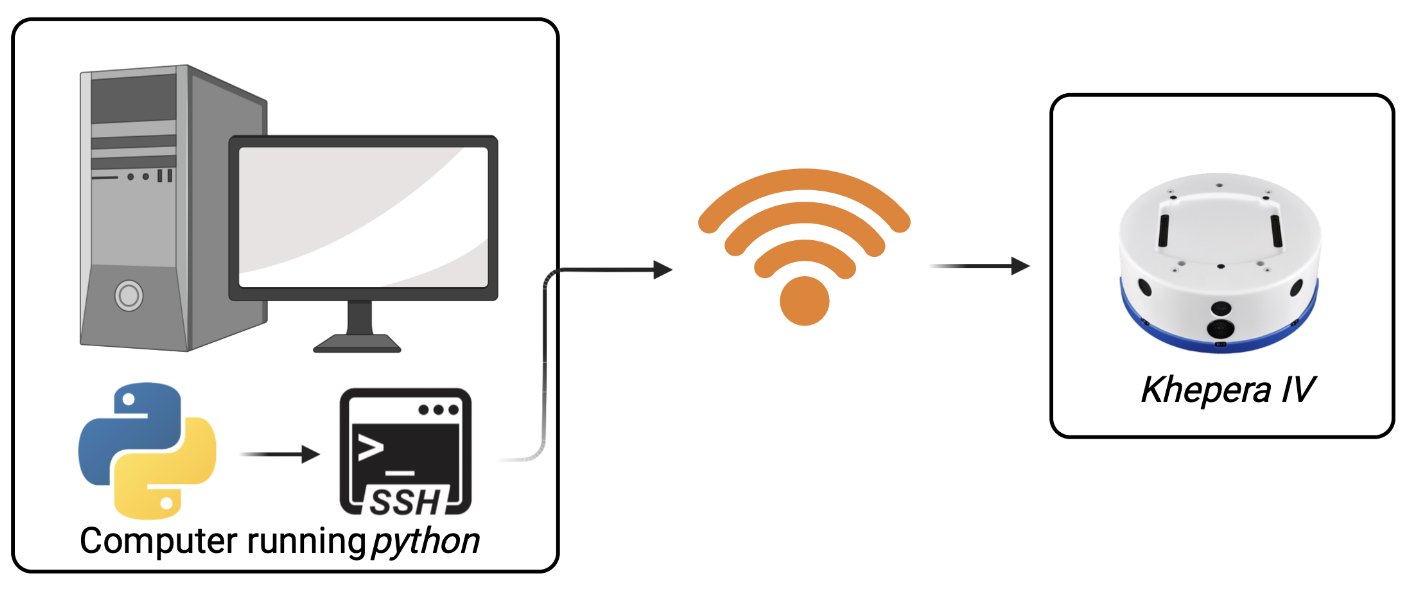
\includegraphics[scale = 0.6]{images/intergration_netwwork.png}
    \caption{This figure shows how the different components of the program integrate with each-other.}

\end{figure}

\subsection{Slice through cube}
\label{fig:hexagona_slice_through_cube}
\begin{figure}[H]
    \centering
    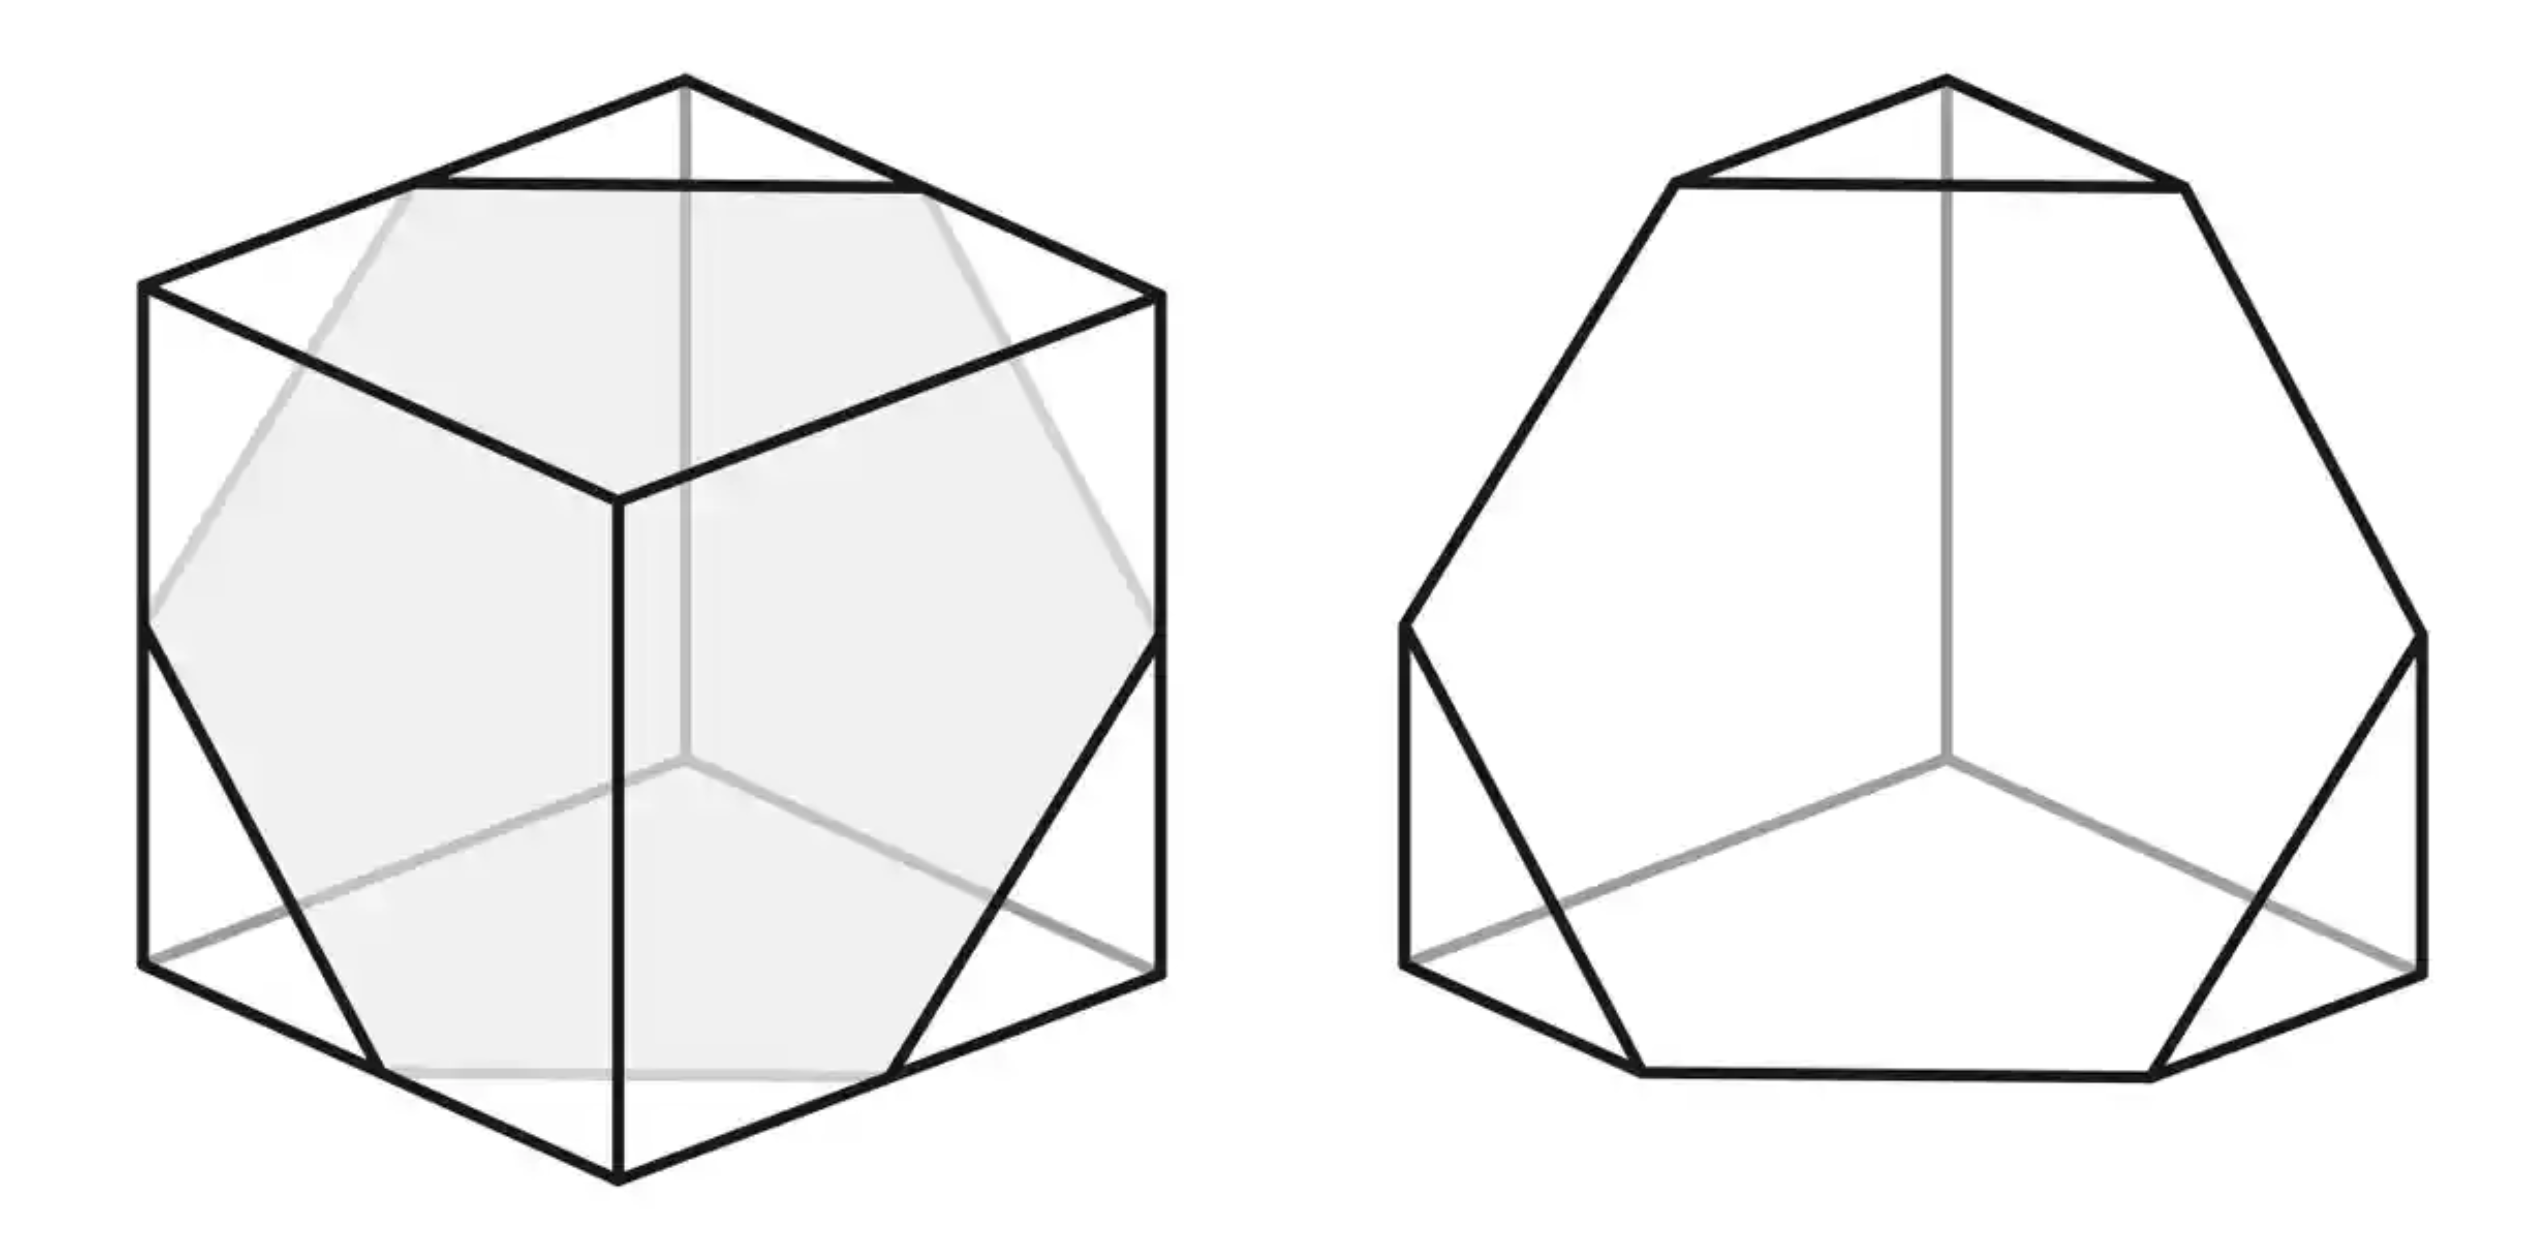
\includegraphics[scale = 0.3]{images/hexagonal_slice_through_cube.png}
    \caption{This is the slice  $x + y + z = 0$ through a cube. From this image it is clear that this plane through 3D space leaves a hexagon. This coordinate system used follows from this observation.}

\end{figure}

\subsection{Truth Table for changing relative position}
\label{table:relative_position_truth_table}

\begin{tabular}{|c||c|c|c|}
    % \centering
    \hline
    \multicolumn{4}{|c|}{Relative Position Truth Table} \\
    \hline
    Axis that is constant & x-axis & y-axis & z-axis \\
    \hline
    Relative Position    & 0 \&  3 & 1 \& 4 & 2 \& 5 \\
    \hline
\end{tabular}


\begin{figure}[H]
\label{table:change_states_of_robot}
\subsection{Truth Table for changing the states of the robots}
\begin{displaymath}
\begin{array}{|c| c||c|}
% |c c|c| means that there are three columns in the table and
% a vertical bar ’|’ will be printed on the left and right borders,
% and between the second and the third columns.
% The letter ’c’ means the value will be centered within the column,
% letter ’l’, left-aligned, and ’r’, right-aligned.
Previously AR & Currently AR & New State\\ % Use & to separate the columns
\hline % Put a horizontal line between the table header and the rest.
True & True & AR\\
True & False & NAR\\
False & True & AR\\
False & False & NNAR\\
\end{array}
\end{displaymath}

\caption{This Table shows how the states of the robot platforms will change based on their previous state and if they have been selected by the animal to become the new animal robot. AR = Animal Robot, NAR = Non Animal Robot and NNAR = Non-Non Animal Robot}
\end{figure}




\subsection{All platform positions the maze must deal with}
\label{fig:all_post_decision_states}
\begin{figure}[H]
    \centering
    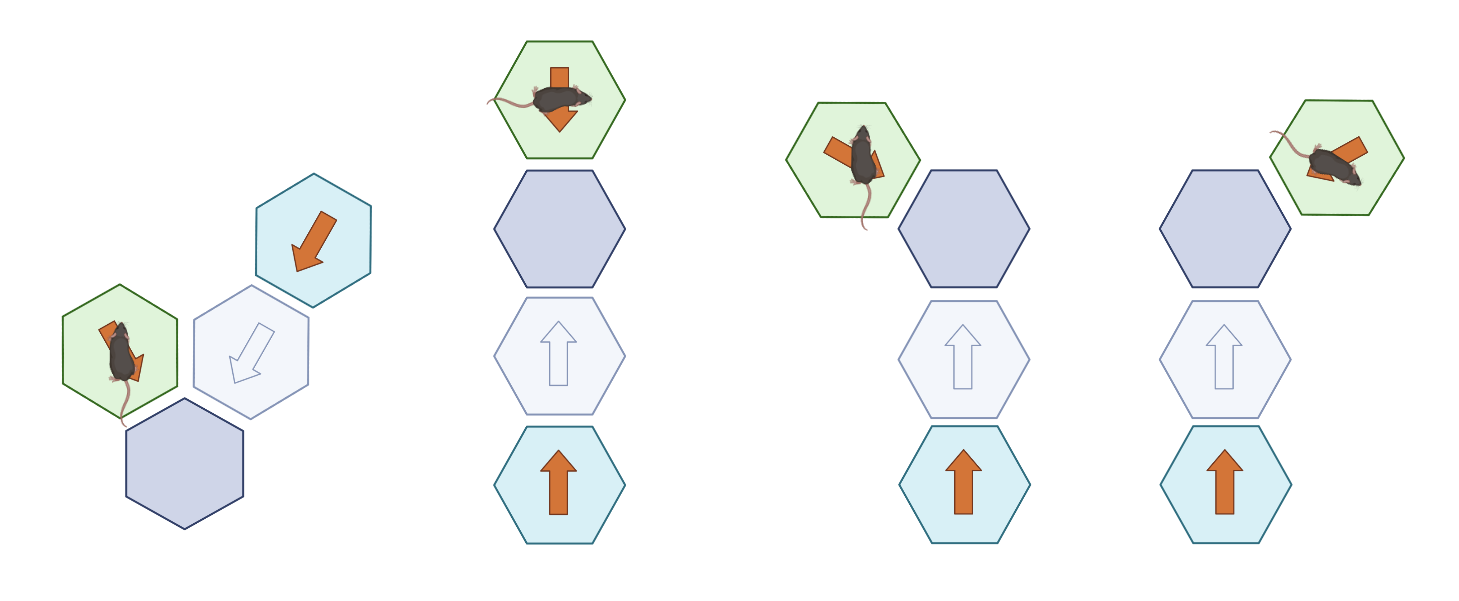
\includegraphics[scale = 0.32]{images/all_post_decision_states.png}
    \caption{This shows all the possible decision states that are possible after the animal has made a decision about which platform to move to, if states which are rotationally symmetric are removed. Since the two most left hand side figures are mirror images of each other, the same algorithm applies to both. This reduces the number of possibilities that need to be handled.}
\end{figure}


\subsection{Example path which the platforms will take through the hexagonal grid}
\label{fig:example_path}
\begin{figure}[H]
    \centering
    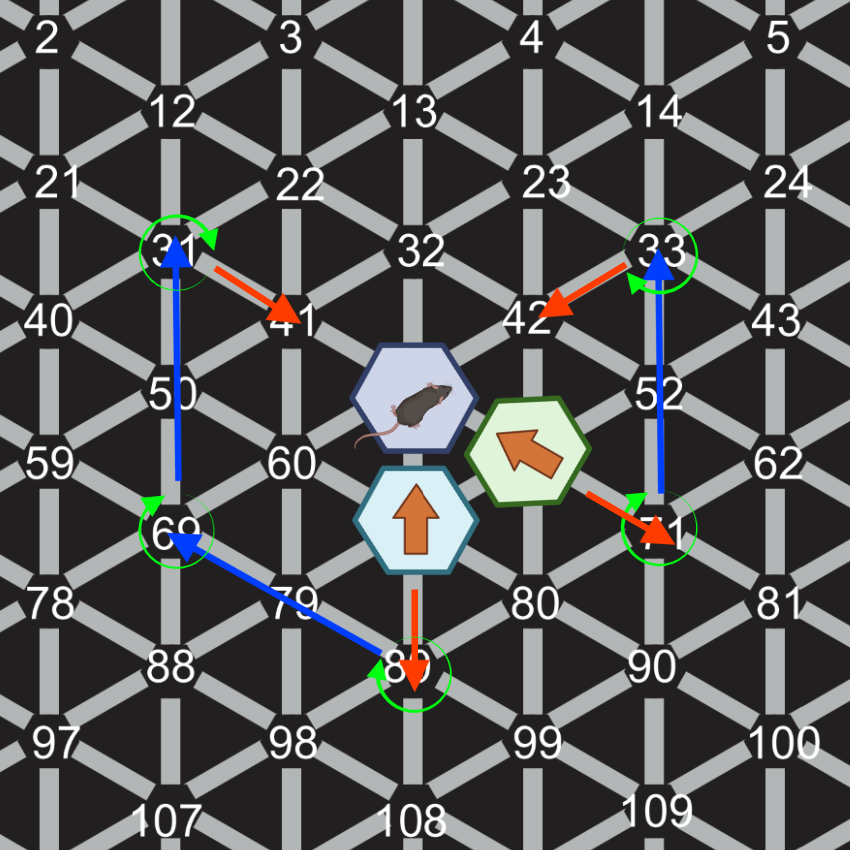
\includegraphics[scale = 0.7]{images/example_path.png}
    \caption{The figure shows the path that the platforms would take around the hexagonal grid.}
\end{figure}



\subsection{Example of consecutive hexagonal platforms colliding}
\label{fig:collision}
\begin{figure}[H]
    \centering
    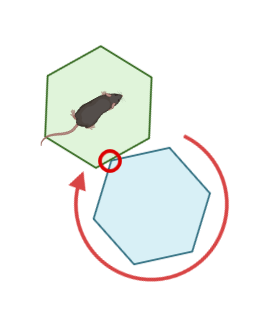
\includegraphics[scale = 0.5]{images/consec_hex_collision .png}
    \caption{This figure shows how two consecutive hexagonal robot are unable to rotate next to each other. The rotating robot (blue) will collide with the stationary one (green)}

\end{figure}

\newpage
\section{Supplementary Material: Functions}

\subsection{Move to Inner Ring}
\label{function:move to inner ring}
\begin{algorithm}
\caption{Implementation of moving the robot to the inner ring}
 \begin{algorithmic}
\REQUIRE Relative Position between \textit{Animal Robot} \AND \textit{Moving Robot}. This will be a number between 0-5, depending on its position around the animal 
\REQUIRE \textit{Inner Ring Steps} List: [-1, -1, -1, 1, 1, 1]
\REQUIRE \textit{Ring Dimension} List: ['x', 'y', 'z', 'x', 'y', 'z']

\STATE $rel pos \leftarrow relative position(\textit{moving_robot})$

\STATE 


    


 \end{algorithmic}
\end{algorithm}

\subsection{Basic moves around the coordinate system}
\label{function:move_around_hex_grid}
\begin{algorithm}
\caption{Function for moving around the hexagonal coordinate space}
 \begin{algorithmic}
 \REQUIRE 'axis' \AND 'step'
   \IF{'axis' is 'x'}
        \STATE$y = y + step$
        \STATE$z = z - step$
        \RETURN $[x, y, z]$
  \ELSIF{'axis' is 'y'}
        \STATE$y = x + step$
        \STATE$z = z - step$
        \RETURN $[x, y, z]$
  \ELSIF{'axis' is 'z'}
        \STATE$y = x + step$
        \STATE$z = y - step$
        \RETURN $[x, y, z]$
   \ENDIF
 \end{algorithmic}
\end{algorithm}

\subsection{Finding relative position}
\label{function:def_relative_position}
\begin{algorithm}[H]
\caption{Function defining the \textit{relative position of a given robot}}
 \begin{algorithmic}
 \REQUIRE \textit{Initial Robot Position Vector, Final Robot Position Vector}
 
 $x, y, z$ is difference in position vectors between \textit{Initial Robot Position Vector} \AND \textit{Final Robot Position Vector}
\IF{$x = 0$ \AND $y = 0$ \AND $z = 0$}
    \RETURN \PRINT{Error Message: Relative Position in not defined here}
\ELSIF{$x = 0$ \AND $x > 0$}
    \RETURN $0$
\ELSIF{$y = 0$ \AND $x > 0$}
    \RETURN $1$
\ELSIF{$z = 0$ \AND $y < 0$}
    \RETURN $2$
\ELSIF{$x = 0$ \AND $x < 0$}
    \RETURN $3$   
\ELSIF{$y = 0$ \AND $x < 0$}
    \RETURN $4$  
\ELSIF{$z = 0$ \AND $y > 0$}
    \RETURN $5$  
\ENDIF
 \end{algorithmic}
\end{algorithm}

\subsection{Change the state of the robots}
\label{function:change_AR_state}
\begin{algorithm}[H]
\caption{Shows the reallocation of the animal robot states after a move has been made by the animal robot}
\function{Reassign robot class}\Comment{Where AR = Animal Robot, NAR = Non-Animal Robot, NNAR = Non-Non-Animal Robot \& State = State of the animal robot}
\begin{algorithmic}
\REQUIRE \textit{New Animal Robot} Class, \textit{Current Robot} Class

\FOR{Each \textit{Robot} in the Maze}
\IF {\textit{Robot} Class is \textit{New Animal} Class \AND the \textit{Robot} Class is \textit{New Animal} Class}
    \STATE \textit{Robot} Class is Animal Robot
\ELSIF {\textit{Robot} Class is \textit{New Animal} Class \AND the \textit{Robot} Class is \textit{New Animal} Class}
    \STATE \textit{Robot} Class is Animal Robot
    
    
\ELSIF {\textit{Robot} Class is \textit{New Non-Animal} Class \AND the \textit{Robot} Class is \textit{New Non-Animal} Class}
    \STATE \textit{Robot} Class is Animal Robot
\ELSIF {\textit{Robot} Class is \textit{New Animal} Class \AND the \textit{Robot} Class is \textit{New Animal} Class}
    \STATE \textit{Robot} Class is Animal Robot
    
\ELSIF {\textit{Robot} Class is \textit{New Non-Non-Animal} Class \AND the \textit{Robot} Class is \textit{New Animal} Class}
    \STATE \textit{Robot} Class is Animal Robot
\ELSIF {\textit{Robot} Class is \textit{New Non-Non-Animal} Class \AND the \textit{Robot} Class is \textit{New Animal} Class}
    \STATE \textit{Robot} Class is Animal Robot
    
    
\ENDIF
\ENDFOR

\end{algorithmic}



\end{algorithm}

\subsection{\textit{Khepera IV} command interpretations}
\label{function:command_interpretation}
\begin{algorithm}
\caption{How the \textit{Khepera IV} interprets command string given to it}
\begin{algorithmic}


% \function{\textit{Khepera IV} command interpretations}\Comment{Input List is a string of numbers}
\REQUIRE Input Command String

\FOR{Each command in \textit{Input Command String}}
    \IF{index of command is even}
        \COMMENT{Interprets the number of turns the robot makes}
        \STATE Rotates the robot 
    \ELSIF{index of command is odd}
        \COMMENT{Interprets the number of moves forwards the robot makes}
        \STATE Moves $command$ number of steps forward
\ENDIF
\ENDFOR
\end{algorithmic}
\end{algorithm}




\subsection{Making Command List}

This function makes commands in the format 'number of turns', 'number of steps', 'number of turns', 'number of steps'...

\label{function:make_command_list}
\begin{algorithm}
\caption{From the path list, making a list of commands interpret-able the \textit{Khepera IV} Robot}
\begin{algorithmic}
\REQUIRE Path List of Coordinates which are consecutive to each-other

\FOR{Each Coordinate in Path List}
    %\Comment{To Handle Turns}
    \STATE Get the position vector between the current position of the robot and the next coordinate
    \STATE Get the Relative position of this position vector
    \IF{Direction of Robot is direction of relative position}
        \STATE Append $0$ to command list
        \COMMENT{No Turns Required}
    \ELSIF {Direction is not relative position}
        \STATE $Turns \leftarrow the different in relative position$
        \COMMENT{Get the number of turns between the desired relative position}
        \STATE Append $Turns$ to Command List 
    
    
    \ELSIF {Position of robot is position in command list}
        \STATE Do nothing
    \ELSIF {Position of robot is not position in command list}
        \STATE Append $1$ to command list
        \COMMENT{Step the robot forward 1 step}
    
    
\ENDIF
\ENDFOR

\RETURN Command List


\end{algorithmic}
\end{algorithm}


\subsection{Making Temporary Movement Network}
\label{function:}
\begin{algorithm}
\caption{}
\begin{algorithmic}

\REQUIRE Movement Network
\REQUIRE Moving Robot

\STATE Temporary Movement Network $\leftarrow$ Movement Network Copy 

\FOR{\textit{Robot} in Maze (excluding Moving Robot)}
    \STATE get the consecutive position of the \textit{robot}
    \STATE Add these positions to list
    
 \FOR{Each position in the list}
       \STATE Remove the position from the Temporary Movement Network
\ENDFOR
\ENDFOR


\RETURN Temporary Movement Network

\end{algorithmic}
\end{algorithm}

\subsection{Get Inner ring coordinates}
\label{function:def_inner_ring}
\begin{algorithm}[H]
\caption{Returns the list of coordinates that are consecutive to the position vector}
\begin{algorithmic}

\REQUIRE Position Vector

inner ring list = [[1, 0, -1], [1, -1, 0], [0, -1, 1],[-1, 0, +1], [-1, 1, 0], [0, 1, -1]]
\FOR{each coordinate in inner ring list}
\STATE new coordinate $\leftarrow$ coordinate + position vector
\STATE append new coordinate to new inner ring list

\ENDFOR
\RETURN new inner ring list
\end{algorithmic}
\end{algorithm}


\subsection{Get Outer ring coordinates}
\label{function:def_outer_ring}
\begin{algorithm}[H]
\caption{Returns the list of coordinates that are two moves away from the position vector}
\begin{algorithmic}

\REQUIRE Position Vector

outer ring = [[2, 0, -2], [2, -1, -1],
                      [2, -2, 0], [1, -2, 1],
                      [0, -2, 2], [-1, -1, 2],
                      [-2, 0, 2], [-2, 1, 1],
                      [-2, 2, 0], [-1, 2, -1],
                      [0, 2, -2], [1, 1, -2]]
\FOR{each coordinate in inner ring list}
\STATE new coordinate $\leftarrow$ coordinate + position vector
\STATE append new coordinate to new outer ring list

\ENDFOR
\RETURN new outer ring list
\end{algorithmic}
\end{algorithm}





%TC:endignore


\end{document}
